\chapter{机器学习理论基础}
\label{chap:statistical-learning-framework}

用一批已标注的邮件训练垃圾邮件分类器，我们希望它也能判断以后收到的新邮件。但训练集上的准确率只检验了分类器对这些训练样本的预测：一个真正抓住了共同规律的分类器，和一个逐条背下训练样本的分类器，都可能在这里拿到高分。要判断学习是否成功，还必须看它们在没见过的邮件上犯多少错误。

把另一批邮件留作测试，可以估计当前这个分类器的错误率。但学习算法的保证还涉及另一层变化：重新抽取一批训练邮件，同一个算法可能选出不同的分类器，表现也随之波动。所以“有限的观测什么时候足以保证未来的错误率低”，取决于三件事：数据是怎么产生的，算法按什么规则选择结果，以及我们允许多大的误差和多高的失败概率。机器学习理论把这三件事写成明确的条件，再在这些条件下证明或否证学习能够成功。

本章始终用同一个只需选一个分界值的邮件分类器作例子，按五个相互衔接的问题展开。第一，学习过程由哪些对象组成，什么叫“学得会”？第~\ref{sec:learning-problem}节分开数据、候选规则、算法和风险，第~\ref{sec:pac-learning}节再把“学得会”写成PAC可学习的正式定义。第二，只追求训练错误最少为什么不够？第~\ref{sec:inductive-bias}节用记忆反例和没有免费的午餐定理说明，缺少对候选规则的限制，任何算法都无法统一成功。第三，限制候选规则要付出什么代价？第~\ref{sec:statistical-model-selection}节逐层拆开风险的来源，并建立后续各章共用的风险比较。第四，限制强弱怎样选择，学习又怎样落实为程序？第~\ref{sec:model-selection}节说明两种选择模型的依据，第~\ref{sec:computable-pac}节在统计保证之上加入停机和资源要求。第五，后续各章往哪里推进？本章最后按表达、优化和泛化整理研究问题，并回顾其发展。

\section{学习问题的组成}
\label{sec:learning-problem}
\label{sec:statistical-learning-problem}

要讨论“未来的错误率”和“重复训练时的成功机会”，先得把学习过程本身说清楚：观测从哪里来，算法从哪些规则里挑选、怎样挑选，挑出的规则又怎样评价。本节依次回答这几个问题。我们会先看到训练记录不足以唯一确定未来的预测，再把这种不确定性写成学习问题；最后比较两种候选规则的范围，直观地看到有的问题随样本增多能够学会，有的问题却无论有多少样本都学不会。“学会”的正式定义留到第~\ref{sec:pac-learning}节给出。

\subsection{观测、输入与数据分布}
\label{sec:learning-problem-data}

设每封邮件已经由一个固定的评分程序给出一个落在$[0,1]$中的可疑程度分数，分数越高表示评分程序认为它越可疑。分类器能读取的这个分数称为\term{预测输入}，记为$x$；人工给出的真实类别称为\term{标签}，记为$y$，约定垃圾邮件为1、正常邮件为0。所有可能的分数组成输入空间$X=[0,1]$，所有标签组成$Y=\{0,1\}$。一封带标签的邮件对应一条观测$z=(x,y)$，所有可能的观测组成观测空间$Z=X\times Y$。预测时只能读到$x$；$y$只在训练记录中提供，用来告诉学习者以前的判断对不对。

邮件的来源有两种随机性。一是哪些分数常见、哪些少见：评分程序给出的分数在不同区间出现的频率不同。二是给定一个分数时邮件属于哪一类：分数同为0.5的两封邮件，可能一封是垃圾邮件、另一封不是。我们用输入与标签的一个联合分布$\mathcal P$同时描述这两种随机性。后一种随机性属于标签本身，即使把同一个分数的邮件重复观察很多次也不会消失；它不是“输入抽得不够多”造成的。学习理论的基本假定是，$\mathcal P$确实存在，却不告诉学习者；学习者只能看到从中抽出的若干封邮件。

训练样本就这样产生：从$\mathcal P$中独立地抽取$n$封邮件，记为$S=((x_1,y_1),\ldots,(x_n,y_n))$。各封邮件彼此独立，并且都服从将来评价时使用的同一个$\mathcal P$，这称为\term{独立同分布}（independent and identically distributed, i.i.d.），写作
\begin{equation}
 S=\bigl((x_1,y_1),\ldots,(x_n,y_n)\bigr)\sim\mathcal P^n.
 \label{eq:training-sample-distribution}
\end{equation}
这里$\mathcal P^n$表示$n$个相互独立、都服从$\mathcal P$的观测的联合分布。将来要分类的新邮件也独立地取自同一个$\mathcal P$。训练邮件和新邮件来自同一个来源，用前者推断后者才有依据。

独立同分布是一个理想化的条件，必须针对具体数据检查。同一封邮件被反复转发，会使训练观测彼此相关；部署之后邮件的类型发生变化，评价时的分布就不再是训练时的分布。前一种情形要重新确定什么算一条独立的观测，后一种情形要加入第~\ref{chap:transfer-learning-theory}章分析的跨域条件。本章及随后的分类与一般学习各章都以独立同分布为起点。

为了能把后面的量都算出来，本节再固定一个教学用的分布：分数在$[0,1]$上均匀分布，即分数落在某个区间的概率等于区间长度；真实的垃圾邮件恰好是分数不低于0.6的邮件，也就是$y=\mathbb I\{x\geq0.6\}$，其中$\mathbb I\{\cdot\}$在括号内条件成立时取1、否则取0。这个分布中给定分数时标签是确定的，只保留了第一种随机性；第~\ref{sec:bayes-risk}节再加入第二种。学习者并不知道这个分布，只看到从中抽出的邮件；我们知道它，只是为了检验学习的结果。

\subsection{假设空间与学习算法}
\label{sec:learning-problem-algorithm}

我们只让分类器学一件事：分界点。分数不低于分界就判为垃圾邮件，低于分界就判为正常邮件，这个分界值称为\term{阈值}（threshold）。每个阈值$t$确定一条分类规则$h_t:X\to Y$。这样一条候选的分类规则就是第~\ref{chap:machine-learning-models}章说的\term{候选模型}，统计学习文献中称为\term{假设}（hypothesis）；所有允许选择的假设合在一起就是候选模型类，统计学习文献中称为\term{假设空间}（hypothesis space），记为$\mathcal H$。只调整阈值时，
\begin{equation}
 \mathcal H_{\mathrm{thr}}=\{h_t:t\in[0,1]\},\qquad
 h_t(x)=\begin{cases}
  1,&x\geq t,\\
  0,&x<t.
 \end{cases}
 \label{eq:threshold-hypothesis-class}
\end{equation}
下标$t$标明采用哪条规则，例如$h_{0.4}$与$h_{0.6}$是其中两个成员。$h_{0.6}(0.5)=0$只陈述“这条规则把分数0.5的邮件判为正常邮件”，这封邮件的真实标签仍须另行观察。

用四封人为构造的邮件看看训练记录能确定什么：分数0.1和0.3是正常邮件，0.7和0.9是垃圾邮件。阈值落在$(0.3,0.7]$中的任何位置，都把前两封判为正常、后两封判为垃圾，训练记录全部分对；这段区间里没有训练邮件，训练标签无法判断阈值该落在哪里。图~\ref{fig:lt4-threshold-email-line}把四封邮件画在数轴上，并画出$h_{0.4}$与$h_{0.6}$判为垃圾邮件的范围；表~\ref{tab:threshold-email-decisions}逐封列出两者的预测。二者分对全部训练邮件，在分数0.5的新邮件上却给出相反的判断。

\begin{figure*}[htbp]
 \centering
 % 第4章：四封训练邮件与两个零训练错误阈值。
% 数据：训练分数 0.1, 0.3（正常，标签 0），0.7, 0.9（垃圾，标签 1）；未标注分数 0.5。
% 零训练错误阈值集合为 (0.3, 0.7]；画出 h_{0.4} 与 h_{0.6} 的判为垃圾区域 [t, 1]。
% 坐标：分数 s 映射到 x = 8 + 90 s（mm）。
\begingroup
\definecolor{FigureBlue}{HTML}{7188A3}\definecolor{FigureBlueFill}{HTML}{E5EAF0}
\definecolor{FigureGreen}{HTML}{829C8B}\definecolor{FigureGreenFill}{HTML}{E8EEE9}
\definecolor{FigureYellow}{HTML}{B4A16F}\definecolor{FigureYellowFill}{HTML}{F1ECDD}
\definecolor{FigureRed}{HTML}{A7787D}\definecolor{FigureRedFill}{HTML}{F0E5E6}
\definecolor{FigureInk}{HTML}{3B4252}\definecolor{FigureMuted}{HTML}{6B7280}
\begin{tikzpicture}[figure picture,x=1mm,y=1mm]
\def\s#1{\fpeval{8+90*#1}}
% zero-training-error band
\fill[FigureYellowFill] (\s{0.3},10.5) rectangle (\s{0.7},26);
\node[figure note,anchor=south] at (\s{0.5},26.5) {零训练错误的阈值都落在 $(0.3,0.7]$};
% axis
\draw[line width=.75pt,draw=FigureStroke,-{Stealth[length=1.6mm]}] (\s{0},14)--(\s{1.06},14);
\foreach \v in {0,0.2,0.4,0.6,0.8,1}{\draw[draw=FigureStroke] (\s{\v},13.2)--(\s{\v},14.8);
  \node[anchor=north,font=\figurefont\scriptsize,text=FigureMuted] at (\s{\v},12.8) {$\v$};}
\node[anchor=west] at (\s{1.06},14) {$x$};
% training emails
\foreach \v in {0.1,0.3}{\draw[draw=FigureBlue,fill=FigureBlueFill,line width=.8pt] (\s{\v},18.5) circle(1.6);
  \node[font=\figurefont\scriptsize] at (\s{\v},22.3) {正常};}
\foreach \v in {0.7,0.9}{\draw[draw=FigureRed,fill=FigureRed,line width=.8pt] (\s{\v},18.5) circle(1.6);
  \node[font=\figurefont\scriptsize] at (\s{\v},22.3) {垃圾};}
% unlabelled email
\draw[draw=FigureInk,fill=white,line width=.8pt,dash pattern=on 1pt off 1pt] (\s{0.5},18.5) circle(1.6);
\node[font=\figurefont\scriptsize] at (\s{0.5},18.5) {?};
% rule bars: predicted spam region [t,1]
\fill[FigureGreenFill] (\s{0.4},4.2) rectangle (\s{1},7.0);
\draw[draw=FigureGreen,line width=1.1pt] (\s{0.4},3.4)--(\s{0.4},7.8);
\node[anchor=east] at (\s{0.4}-1,5.6) {$h_{0.4}$};
\fill[FigureBlueFill] (\s{0.6},-2.2) rectangle (\s{1},0.6);
\draw[draw=FigureBlue,line width=1.1pt] (\s{0.6},-3.0)--(\s{0.6},1.4);
\node[anchor=east] at (\s{0.6}-1,-0.8) {$h_{0.6}$};
\node[figure note,anchor=west] at (\s{1}+1.5,2.4) {浅色段：\\判为垃圾};
\draw[draw=FigureMuted,line width=.5pt,dash pattern=on 1pt off 1.2pt] (\s{0.5},16.6)--(\s{0.5},-3.5);
\end{tikzpicture}
\endgroup

 \caption{数轴上的四封训练邮件与两个阈值规则。空心点为正常邮件，实心点为垃圾邮件，虚线圈为尚未标注的分数0.5。浅黄色区间内的任何阈值都分对全部训练邮件；下方两条色带分别是$h_{0.4}$与$h_{0.6}$判为垃圾邮件的分数范围，二者在0.5处给出相反的预测。}
 \label{fig:lt4-threshold-email-line}
\end{figure*}

\begin{table}[htbp]
 \centering
 \begin{tabular}{cccc}
  \toprule
  邮件分数 & 已知类别 & 阈值0.4的预测 & 阈值0.6的预测\\
  \midrule
  0.1 & 正常 & 正常 & 正常\\
  0.3 & 正常 & 正常 & 正常\\
  0.7 & 垃圾 & 垃圾 & 垃圾\\
  0.9 & 垃圾 & 垃圾 & 垃圾\\
  \midrule
  0.5 & 尚未标注 & 垃圾 & 正常\\
  \bottomrule
 \end{tabular}
 \caption{四封构造的训练邮件与一封未标注邮件上的阈值预测。两个阈值分对全部训练记录，却在分数0.5处产生分歧；末行没有真实标签，故不能据它判断谁正确。}
 \label{tab:threshold-email-decisions}
\end{table}

训练记录既然不能唯一确定规则，就需要一个从记录到规则的选择方法。\term{学习算法}读入训练样本，从$\mathcal H$中交出一条规则。把这个从样本到规则的对应记为$A$，一次训练得到的规则写成$\hat h=A(S)$，称为训练模型。二者要分开：$A$是“任给一份样本，怎样选规则”的整套做法，$\hat h$只是这一份样本下选出的具体规则。说“这个模型”时指的是$\hat h$，说“这个学习器”时指的是$A$。

最自然的选择原则是数一数每个阈值在训练样本上分错几封，选分错最少的，这称为经验风险最小化，正式定义在下一小节给出。这个原则只规定了要选训练错误最少的规则，还没有交代三件事，而它们都属于算法的一部分。其一，并列时选哪个：上面的$(0.3,0.7]$中有无穷多个同样好的阈值，算法必须规定例如选其中最小者，或者选区间中点。其二，近似求解：候选太多、无法逐一检查时，算法可能只找到训练错误接近最少的规则。其三，内部随机性：算法可以在并列者中随机挑一个，这时用一个独立于样本的随机量$U$记录这部分随机性，输出写作$A(S,U)$。两个都遵守“训练错误最少”的算法，可以因为这三点不同而交出不同的规则；训练记录上表现最好，也还不说明交出的规则在新邮件上表现好。

\subsection{经验风险、期望风险与泛化差}
\label{sec:learning-problem-risk}

要比较$h_{0.4}$和$h_{0.6}$，先要给每次预测计分。\term{损失}（loss）为一次预测计分；当前对两种误判同等看待，判错记1、判对记0，这就是\term{零一损失}（zero-one loss）：
\begin{equation}
 \ell_{01}(h(x),y)=\begin{cases}
  1,&h(x)\neq y,\\
  0,&h(x)=y.
 \end{cases}
 \label{eq:zero-one-loss}
\end{equation}
如果误删正常邮件的代价更大，就要换用不对称的计分；本章先固定零一损失。

损失可以按两种方式取平均。我们真正关心的是随机到来的一封新邮件被判错的概率：按$\mathcal P$对损失取平均，得到$h$的\term{期望风险}。零一损失只取0或1，所以它就是分类错误的概率：
\begin{equation}
 R_{\mathcal P}(h)
 =\mathbb E_{(x,y)\sim\mathcal P}[\ell_{01}(h(x),y)]
 =\mathbb P_{(x,y)\sim\mathcal P}(h(x)\neq y).
 \label{eq:population-classification-risk}
\end{equation}
学习者不知道$\mathcal P$，算不出这个平均，但能算样本上的平均，即\term{经验风险}：
\begin{equation}
 \hat R_S(h)=\frac1n\sum_{i=1}^n\ell_{01}(h(x_i),y_i).
 \label{eq:empirical-classification-risk}
\end{equation}
分子是样本中的错误数，除以$n$得到这份样本上的错误比例。下标标出了各自依赖什么：$R_{\mathcal P}$依赖总体分布，$\hat R_S$依赖已经观察到的样本。$S$取训练样本时，$\hat R_S$是训练错误率；换成独立的测试样本时，它是对未来错误率的一次估计。

在教学分布下，期望风险可以直接算出。阈值$t<0.6$时，规则$h_t$把$[t,0.6)$上的正常邮件误判为垃圾邮件；$t>0.6$时，把$[0.6,t)$上的垃圾邮件误判为正常邮件。分数均匀分布，误判区间的概率等于它的长度，所以
\begin{equation}
 R_{\mathcal P}(h_t)=|t-0.6|.
 \label{eq:threshold-teaching-risk}
\end{equation}
于是$h_{0.6}$的风险为0，$h_{0.4}$的风险为0.2。四封训练邮件上二者的经验风险都是零，它们之间的差别来自我们知道的分布，而不是训练数据。

有了经验风险，上一小节的选择原则可以写成定义。

\begin{definition}[经验风险最小化]
\label{def:erm-learning-rule}
\term{经验风险最小化}（empirical risk minimization, ERM）是在给定假设空间中，选择
训练样本平均损失最小的假设作为学习结果。用$A_{\mathrm{ERM}}$表示这种学习算法，则
\begin{equation}
 A_{\mathrm{ERM}}(S)\in\argmin_{h\in\mathcal H}\hat R_S(h).
 \label{eq:erm-learning-rule}
\end{equation}
这里$\argmin$表示所有达到最小经验风险的假设组成的集合。若最小值不能取得，可以
要求输出的经验风险与下确界相差不超过一个给定容差。
\end{definition}

式中的“$\in$”表示并列时可以任选其中一个，ERM本身没有规定选哪一个；阈值0.4和0.6就是一对并列的经验最优解。

经验风险与期望风险之差$R_{\mathcal P}(h)-\hat R_S(h)$称为\term{泛化差}（generalization gap），可正可负。对一条事先固定、与样本无关的规则，样本越多，经验风险越接近期望风险，这是大数定律的结论。但训练模型$\hat h=A(S)$是看过$S$才选出的，算法专挑在这份样本上表现好的规则，它的训练错误率往往偏低；$\hat h$与$S$相互依赖，“固定规则、随机样本”的估计不能直接套用。后续各章用容量、稳定性和信息依赖分析泛化，共同处理的正是这种输出与训练数据之间的依赖。

\subsection{一次训练与重复训练的评价}
\label{sec:learning-problem-learnable}

有了这些对象，就可以提出本章的核心问题：样本越来越多时，算法交出的规则能否以越来越大的把握，达到很低的期望风险？回答它之前，先分清“评价一次训练”与“评价一个算法”这两件事，再分别看阈值规则和不加限制的规则，两者给出相反的答案。

\paragraph{两层随机性}
固定训练模型$\hat h$后，$R_{\mathcal P}(\hat h)$只对新邮件取平均，是一个确定的数；用一批独立的测试邮件可以估计它。但重新抽一份训练样本，同一个算法可能选出不同的规则：一份样本恰好有许多邮件落在0.6附近，另一份恰好缺少它们，学到的阈值就不同。所以$R_{\mathcal P}(A(S))$本身随$S$变化，是一个随机变量。图~\ref{fig:learning-two-randomness}把两层分开画出：右侧对新观测取平均，评价的是已经训练好的这一个模型；左侧对训练样本重新抽样，评价的是学习算法。学习的保证要控制的，是左侧这一层变化造成高风险结果的概率。算法若使用内部随机数$U$，这部分随机性也要计入。

\begin{figure*}[htbp]
  \centering
  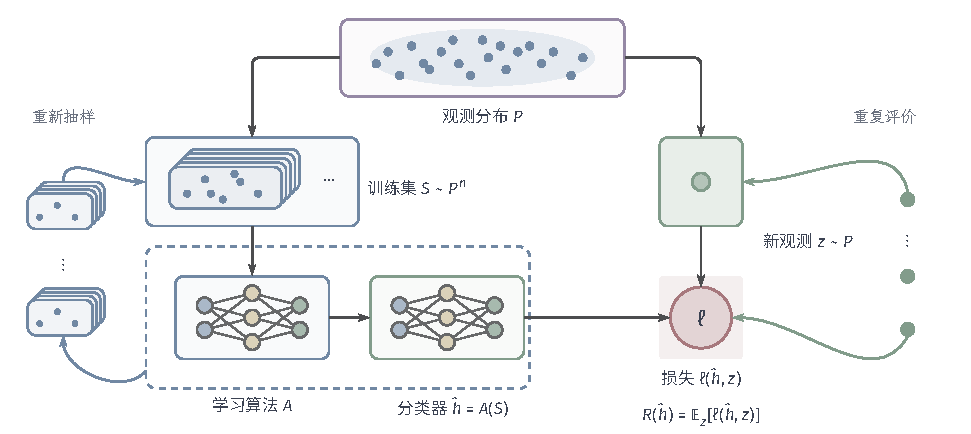
\includegraphics[width=164.600mm]{figures/06-foundations/02-learning-theory/tikz/learning-theory-two-randomness/figure.pdf}
  \caption{两层随机性的评价对象。固定训练模型后，右侧新观测的平均损失给出期望风险；左侧重新抽样则改变输出，学习保证控制这种变化造成高风险结果的概率。}
 \label{fig:learning-two-randomness}
\end{figure*}

\paragraph{阈值规则}
在教学分布下，正常邮件的分数都小于0.6，垃圾邮件的分数都不低于0.6。训练错误为零的阈值，必须大于样本中正常邮件的最高分数、且不超过垃圾邮件的最低分数，所以这些阈值都落在包含0.6的一段区间里。图~\ref{fig:lt4-threshold-squeeze}画出三份构造的样本：4封邮件时，零错误区间是$(0.45,0.71]$；8封时缩到$(0.55,0.66]$；16封时只剩$(0.58,0.62]$。样本越多，0.6两侧越可能各有一封邮件靠得很近，这段区间就被夹得越紧。

\begin{figure*}[htbp]
 \centering
 % 第4章：零训练错误阈值区间随样本增多被夹紧。
% 教学分布：x ~ Uniform[0,1]，y = 1{x >= 0.6}。三行是构造的示意样本（非随机抽样结果）：
%   n=4 : 正常 0.12, 0.45；垃圾 0.71, 0.88            -> 区间 (0.45, 0.71]
%   n=8 : 正常 0.08, 0.27, 0.43, 0.55；垃圾 0.66, 0.74, 0.83, 0.95 -> 区间 (0.55, 0.66]
%   n=16: 正常 0.04,0.11,0.19,0.26,0.33,0.41,0.49,0.58；垃圾 0.62,0.67,0.72,0.79,0.84,0.90,0.93,0.98 -> (0.58, 0.62]
% 竖带为 [0.6-eps, 0.6+eps]，eps = 0.05；风险 |t-0.6| > eps 恰为阈值落在带外。
% 坐标：分数 s 映射到 x = 14 + 88 s（mm）。
\begingroup
\definecolor{FigureBlue}{HTML}{7188A3}\definecolor{FigureBlueFill}{HTML}{E5EAF0}
\definecolor{FigureGreen}{HTML}{829C8B}\definecolor{FigureGreenFill}{HTML}{E8EEE9}
\definecolor{FigureYellow}{HTML}{B4A16F}\definecolor{FigureYellowFill}{HTML}{F1ECDD}
\definecolor{FigureRed}{HTML}{A7787D}\definecolor{FigureRedFill}{HTML}{F0E5E6}
\definecolor{FigureInk}{HTML}{3B4252}\definecolor{FigureMuted}{HTML}{6B7280}
\begin{tikzpicture}[figure picture,x=1mm,y=1mm]
\def\s#1{\fpeval{14+88*#1}}
% epsilon band around the true threshold
\fill[FigureGreenFill] (\s{0.55},-1) rectangle (\s{0.65},33);
\draw[draw=FigureGreen,line width=.8pt] (\s{0.6},-1)--(\s{0.6},33);
\node[figure note,anchor=south] at (\s{0.6},33.3) {真实分界 $0.6$ 及其两侧 $\varepsilon=0.05$};
% one row: #1 = y, #2 = label, #3 = negatives, #4 = positives, #5 = left end, #6 = right end
\newcommand{\squeezerow}[6]{%
  \draw[draw=FigureStroke,line width=.6pt] (\s{0},#1)--(\s{1},#1);
  \fill[FigureYellow] (\s{#5},{#1-1.1}) rectangle (\s{#6},{#1+1.1});
  \foreach \v in {#3}{\draw[draw=FigureBlue,fill=FigureBlueFill,line width=.7pt] (\s{\v},{#1+3}) circle(1.1);}
  \foreach \v in {#4}{\draw[draw=FigureRed,fill=FigureRed,line width=.7pt] (\s{\v},{#1+3}) circle(1.1);}
  \node[anchor=east] at (\s{0}-1.5,#1+1.5) {#2};
  \node[anchor=west,font=\figurefont\scriptsize] at (\s{1}+1.5,#1+1.5) {$(#5,#6]$};}
\squeezerow{25}{$n=4$}{0.12,0.45}{0.71,0.88}{0.45}{0.71}
\squeezerow{14}{$n=8$}{0.08,0.27,0.43,0.55}{0.66,0.74,0.83,0.95}{0.55}{0.66}
\squeezerow{3}{$n=16$}{0.04,0.11,0.19,0.26,0.33,0.41,0.49,0.58}{0.62,0.67,0.72,0.79,0.84,0.90,0.93,0.98}{0.58}{0.62}
\foreach \v in {0,0.2,0.4,0.6,0.8,1}{\node[anchor=north,font=\figurefont\scriptsize,text=FigureMuted] at (\s{\v},-1.5) {$\v$};}
\node[anchor=west,font=\figurefont\scriptsize,text=FigureMuted] at (\s{1}+1.5,-3.2) {零错误区间};
\end{tikzpicture}
\endgroup

 \caption{零训练错误阈值的区间随样本增多被夹紧。三行是教学分布下构造的示意样本（不是随机抽样的结果），空心点为正常邮件，实心点为垃圾邮件；粗色段是该样本上训练错误为零的阈值集合，右侧写出其端点。绿色竖线为真实分界0.6，浅绿带为其两侧宽0.05的范围；色段伸出浅绿带时，算法可能交出风险超过0.05的阈值。}
 \label{fig:lt4-threshold-squeeze}
\end{figure*}

把这个观察写成概率。算法无论在零错误区间中怎样选，选出的$\hat t$都满足：若$\hat t<0.6-\varepsilon$，则没有训练邮件落在$[0.6-\varepsilon,0.6)$中，否则那封正常邮件的分数会超过$\hat t$而被判错；若$\hat t>0.6+\varepsilon$，则没有训练邮件落在$[0.6,0.6+\varepsilon]$中。由式~\eqref{eq:threshold-teaching-risk}，风险超过$\varepsilon$恰好意味着$\hat t$偏离0.6超过$\varepsilon$，于是对$0<\varepsilon<0.4$，
\begin{equation}
 \mathbb P_{S\sim\mathcal P^n}\bigl(R_{\mathcal P}(h_{\hat t})>\varepsilon\bigr)
 \leq2(1-\varepsilon)^n\leq2e^{-n\varepsilon}.
 \label{eq:threshold-teaching-sample}
\end{equation}
每个长为$\varepsilon$的区间里没有训练邮件的概率是$(1-\varepsilon)^n$，两侧各一个区间，用并集界得到因子2；最后一步用了$1-u\leq e^{-u}$。$\varepsilon\geq0.4$时$0.6+\varepsilon\geq1$，阈值不可能偏到右侧那么远，只剩左侧一种失败方式（$\varepsilon\geq0.6$时连它也不可能），上式仍成立。要以至少99\%的把握得到风险不超过5\%的阈值，令$2e^{-0.05n}\leq0.01$，解得$n\geq106$。总有小概率抽到的邮件都远离0.6，这就是右端那个随$n$迅速变小、却不为零的失败概率。

\paragraph{不加限制的规则}
现在放宽候选范围：允许任何从分数到标签的函数。上面四封训练邮件仍然都能分对，可是它们对分数0.5的新邮件说明不了任何事情：有的函数分对四封训练邮件并把0.5判为垃圾邮件，有的同样分对它们却把0.5判为正常邮件，两者都在候选范围内。分数连续分布，新邮件几乎不可能恰好与某封训练邮件同分，所以几乎每封新邮件都会遇到这种歧义。多抽几封邮件也无济于事：新样本只确定它们自己的标签，对其余分数仍然没有约束。

\paragraph{从直观对照到正式要求}
两个例子对照出“学得会”的意思：存在一个学习算法，无论真实来源是允许范围中的哪一个，只要样本足够多，它都能以很大的把握交出风险接近最好水平的规则；而且“足够多”是多少，可以事先算出来，不依赖那个未知的来源。按这个标准，阈值规则看来学得会，不加限制的规则学不会。区别不在候选的个数，二者都含无穷多条规则；区别在于已见的标签能否约束未见输入上的预测。阈值规则一旦把分数0.7判为垃圾邮件，所有更高分数也必须判为垃圾邮件；不加限制的规则在不同分数之间没有任何联系。

预先限定候选规则的形状、或规定在多个候选之间怎样取舍，称为\term{归纳偏置}（inductive bias）。白话地说，它是数据之外由我们补充的假定，使算法能把已有判断延伸到没见过的输入上；它的代价是，若真实规律不符合这一假定，算法就会系统地出错。奥卡姆剃刀表达“优先采用更简单解释”的想法：一个分界值就能指定一条阈值规则，而不加限制的规则要逐个分数写出答案。不过描述长短取决于编码方式，单凭“简单”推不出学得会，还必须证明这种限制怎样控制了统计误差，第~\ref{chap:binary-learnability}章会给出这类证明。

上面的描述还有几处不够确切：风险“接近最好水平”是和谁比、允许差多少，“很大的把握”是多大，“无论真实来源是哪一个”又指哪些来源。下一节逐一回答这些问题，给出可学习的正式定义；“不加限制的规则学不会”这一判断，则要到第~\ref{sec:no-free-lunch}节才能证明。

\section{PAC学习}
\label{sec:pac-learning}

本节把“学得会”写成可以证明或否证的陈述。上一节留下的四个问题各对应定义中的一个要素。第一，和谁比？以假设空间中的最低期望风险为基准；即使空间里没有完美的规则，也能衡量算法离最好的候选还有多远。第二，允许差多少？用容差$\varepsilon$限制输出风险比基准高出的部分。第三，有多大把握？训练样本是随机的，总可能抽到一份很不典型的样本，所以只要求成功的概率至少为$1-\delta$。第四，对哪些来源成立？算法不知道真实的$\mathcal P$，所以同一个算法、同一个样本量必须对允许范围内的每个分布都有效。

\term{PAC学习}（probably approximately correct learning，概率近似正确学习）把这四点写在一起：名称里的“近似正确”对应$\varepsilon$允许的风险偏差，“概率”对应至少$1-\delta$的成功率。例如要求“以至少99\%的概率，得到一个未来错误率不超过5\%的分类器”，就是取$\delta=0.01$、$\varepsilon=0.05$。其中5\%约束的是某一次训练得到的分类器在总体上的错误概率，99\%约束的是“抽一批样本再训练”这个随机过程成功的机会；它既不要求训练集里每条记录都分对，也不要求每一批未来邮件的实际错误率都不超过5\%。

基准取零风险还是类内最低风险，取决于假设空间里是否存在零风险的规则，由此分出可实现与不可知两种情形。两者先在二分类和零一损失下给出；随后比较样本复杂度与几种保证的强弱，最后在第~\ref{sec:pac-general-form}节写成对一般任务都适用的形式。

\subsection{可实现PAC学习}
\label{sec:pac-realizable}

先假设$\mathcal H$中确实存在一个总体零错误的规则。这暂时排除了标签噪声和假设空间表达不足造成的不可避免错误，让我们集中分析一个问题：正确答案已经在假设空间里时，有限的观测是否足以把它（或另一个风险同样低的规则）选出来。

\begin{definition}[可实现性]
\label{def:realizability}
若存在$h^\star\in\mathcal H$满足$R_{\mathcal P}(h^\star)=0$，即$h^\star$以概率1正确预测
标签，就称分布$\mathcal P$对假设空间$\mathcal H$是\term{可实现的}（realizable）。
\end{definition}

教学分布由阈值0.6确定标签，而$h_{0.6}\in\mathcal H_{\mathrm{thr}}$，所以它对阈值空间可实现。这里要求的是总体中存在零风险的规则，与有限训练样本恰好无冲突是两回事。如果同一个分数可以对应两种标签，分数本身就不支持零错误预测；反过来，一张训练表上碰巧没有冲突标签，只说明有限观测没暴露矛盾，不能据此确认可实现性。

\begin{definition}[可实现PAC可学习]
\label{def:realizable-pac}
若存在学习算法$A$及函数$m_{\mathcal H}:(0,1)^2\to\mathbb N$，使对任意
$\varepsilon,\delta\in(0,1)$、任意对$\mathcal H$可实现的分布$\mathcal P$及任意
$n\geq m_{\mathcal H}(\varepsilon,\delta)$都有
\begin{equation}
 \mathbb P_{S\sim\mathcal P^n}
 \left(R_{\mathcal P}(A(S))\leq\varepsilon\right)\geq1-\delta,
 \label{eq:pac-guarantee}
\end{equation}
就称$\mathcal H$是可实现PAC可学习的。算法使用内部随机数时，概率同时对$S$与$U$计算。
\end{definition}

式~\eqref{eq:pac-guarantee}要从内往外读。内层评价一次训练：$A(S)$是这次训练得到的分类器，$R_{\mathcal P}(A(S))\leq\varepsilon$是“这次成功”的事件。外层再对训练样本的随机抽取取概率，要求成功的概率至少为$1-\delta$。误差容限$\varepsilon$限制的是模型的总体风险，失败概率$\delta$限制的是重复训练时不成功的机会；二者不是两种分类错误率。

量词的顺序同样要紧：先固定同一个算法$A$，再对每组$\varepsilon,\delta$确定样本门槛$m_{\mathcal H}(\varepsilon,\delta)$，随后才要求全部可实现分布都受保证。$m_{\mathcal H}$只能依赖$\varepsilon$、$\delta$和$\mathcal H$，不能随未知的分布改变。若允许先看到分布再定样本量，结论就只对那个分布成立，不再是对未知来源的保证。PAC这一形式化由Valiant提出，本章采用统计学习教材中的分布无关表述\scite{valiant1984,shalevshwartz2014}。

上一节的式~\eqref{eq:threshold-teaching-sample}只对教学分布算出了样本量；定义要求的是一个对全部可实现分布都够用的样本量。第~\ref{chap:binary-learnability}章将证明阈值空间满足这一更强的要求。

\subsection{不可知PAC学习}
\label{sec:pac-agnostic}

现实中，假设空间里往往没有零风险的规则，或者无法确认有没有。零风险不可达有两种来源。一是输入信息不足：即使完全知道分布，同一分数仍可能以正概率对应两种标签，这种错误不可避免。二是假设空间表达不了所需的预测关系，例如垃圾邮件的分数落在两段分离的区间时，单个阈值无论放在哪里都会出错。第~\ref{sec:statistical-model-selection}节会分别刻画这两者。

无论是哪种来源，都不能再指望零风险，于是改用$\mathcal H$内的最低风险作为基准。空间中未必有恰好达到它的成员，例如各规则的风险依次为$0.08+0.1/k$（$k=1,2,\ldots$）时，可以无限趋近0.08却取不到它，所以用下确界记录这个水平：
\begin{equation}
 R_{\mathcal P,\mathcal H}^\star=\inf_{h\in\mathcal H}R_{\mathcal P}(h).
 \label{eq:best-in-class-risk}
\end{equation}
学习输出的期望风险与$R_{\mathcal P,\mathcal H}^\star$之差称为\term{超额期望风险}（excess risk），简称超额风险。它衡量的是相对这一基准的差距，而不是总风险。假设$\mathcal H$的最低期望风险是8\%，那么要求恰当学习器达到2\%的总风险在这个空间里根本不可能；合理的要求是让它只比8\%多2个百分点。

\begin{definition}[不可知PAC可学习]
\label{def:agnostic-pac}
若存在学习算法$A$及函数$m_{\mathcal H}^{\mathrm{agn}}:(0,1)^2\to\mathbb N$，使对任意
$\varepsilon,\delta\in(0,1)$、任意$X\times Y$上的联合分布$\mathcal P$及任意
$n\geq m_{\mathcal H}^{\mathrm{agn}}(\varepsilon,\delta)$都有
\begin{equation}
 \mathbb P_{S\sim\mathcal P^n}\left(
 R_{\mathcal P}(A(S))\leq R_{\mathcal P,\mathcal H}^\star+\varepsilon
 \right)\geq1-\delta,
 \label{eq:agnostic-pac-guarantee}
\end{equation}
就称$\mathcal H$是\term{不可知PAC可学习的}（agnostic PAC learnable）。
\end{definition}

这种设定称为\term{不可知设定}（agnostic setting）：它不承诺零风险的规则在$\mathcal H$内，也不预先限制噪声的形式；训练标签可用、样本独立同分布这两个条件仍然保留。可实现分布也包含在覆盖范围里：它的类内最低风险为零，式~\eqref{eq:agnostic-pac-guarantee}就退化为式~\eqref{eq:pac-guarantee}。所以不可知学习扩大的是需要统一处理的分布范围，而不是放宽了成功标准。类内最低风险只用于评价，算法事先不需要知道它。

“噪声”指什么，取决于评价时使用哪种标签。如果观测到的标签本身就是要预测的$y$，标签中的随机性就是分布$\mathcal P$的一部分，不可知设定已经把它包括在内；如果训练用的标签和评价用的标签不是同一种，例如用廉价标签训练、用专家标签评价，就要额外规定两种标签之间的关系，上面的同分布保证不能直接套用，也不能只用“不可知”一词把这种差别覆盖过去。

\subsection{样本复杂度与保证的强弱}
\label{sec:pac-sample-complexity}

两个PAC定义只要求存在某个够用的样本量，而实际关心的是“最少要多少”。若$m_{\mathcal H}$够用，任何更大的函数也够用。对给定的$\varepsilon$和$\delta$，在所有允许的算法中，能使保证从某个样本量起一直成立的最小门槛，称为\term{样本复杂度}（sample complexity），它衡量这个学习问题本身需要多少数据。

证明一个上界与证明一个下界的工作量不同。要说明$m$个样本足够，只需展示一个算法，并证明它在$m$个样本下对每个允许分布都成功；要说明少于$m'$个样本不够，则必须排除样本不足时的\emph{所有}允许算法，通常要构造一个使任何算法都失败的分布，第~\ref{sec:no-free-lunch}节就是这样的论证。反解风险界得到的样本数是上界，不自动最优。以教学分布为例：由$2(1-\varepsilon)^n\leq\delta$求得$\varepsilon=0.05$、$\delta=0.01$时$n\geq104$，而由更宽松的$2e^{-n\varepsilon}\leq\delta$求得$n\geq106$。两个数都保证成功，后者只是因为多用了一次不等式放缩而偏大；这里的差别很小，但在复杂的界中，放缩的累积可能使样本数相差很多倍。

保证还按“覆盖哪些来源”分强弱。PAC要求一个样本门槛覆盖整个允许来源族，称为\emph{分布无关}的保证。另一种较弱的要求只对每个固定分布谈收敛：样本量趋于无穷时，输出的超额风险依概率趋于零，这称为算法的\term{一致性}（consistency）。一致性允许所需的样本量随分布变化：对某个分布，几百封邮件就够；对另一个分布，可能要几百万封，而且事先无法知道面对的是哪一个。所以一致性不能推出PAC可学习。

保证还按“控制什么量”分强弱。PAC控制的是失败概率，即高风险结果出现的机会；另一类结论只控制平均风险$\mathbb E_SR_{\mathcal P}(A(S))$。仍用教学分布：对式~\eqref{eq:threshold-teaching-sample}的尾概率积分，
\[
 \mathbb E_SR_{\mathcal P}(h_{\hat t})
 =\int_0^1\mathbb P\bigl(R_{\mathcal P}(h_{\hat t})>\varepsilon\bigr)\,\mathrm d\varepsilon
 \leq\int_0^\infty2e^{-n\varepsilon}\,\mathrm d\varepsilon=\frac2n,
\]
第一步用了取值于$[0,1]$的随机变量的期望等于其尾概率的积分。平均风险以$2/n$的速度下降，并不直接告诉我们“以99\%的把握风险不超过5\%”需要多少样本。从平均量回到失败概率需要额外的论证，第~\ref{sec:risk-comparison}节给出其条件；后续章节也不能只因为某个平均量趋于零，就声称已经证明了原定的PAC结论。

\subsection{一般损失、比较空间与输出空间}
\label{sec:pac-general-form}
\label{sec:learning-problem-general-risk}

后续各章还要处理多分类、回归、聚类等任务，评价方式相同，变的只是观测和计分。两个例子说明需要推广什么。回归中，观测是$z=(x,y)$且$y$为实数，被评价的对象是一个实值预测函数$f$，常用平方损失$(f(x)-y)^2$计分；聚类中，观测只有一个点$z$，被评价的对象是一组中心$\{c_1,\ldots,c_k\}$，损失可以取$z$到最近中心的平方距离。后一个例子里根本没有“分类器”，也没有标签。

于是把一条观测一般地记为$z$，所有可能的观测组成观测空间$Z$；被评价的对象称为\emph{决策}，记为$w$，监督预测中它就是一条预测规则，聚类中则是一组中心；损失函数$\ell(w,z)$表示用决策$w$处理观测$z$时付出的代价，数值越小越好。二分类中$z=(x,y)$，决策是分类器$h$，损失取零一损失$\ell(h,(x,y))=\ell_{01}(h(x),y)$。风险的两种平均沿用同样的形式。

\begin{definition}[一般学习问题的期望风险]
\label{def:general-population-risk}
设$\mathcal P$是$Z$上的分布。对决策$w$，若$\ell(w,\cdot)$在$\mathcal P$下可积，则$w$的期望风险为
\[
 R_{\mathcal P}(w)=\mathbb E_{z\sim\mathcal P}\ell(w,z).
\]
\end{definition}

\begin{definition}[一般学习问题的经验风险]
\label{def:general-empirical-risk}
给定样本$S=(z_1,\ldots,z_n)\in Z^n$，决策$w$的经验风险为
\begin{equation}
 \hat R_S(w)=\frac1n\sum_{i=1}^n\ell(w,z_i).
 \label{eq:general-risk}
\end{equation}
\end{definition}

被推广的只是风险的定义形式；“平均损失等于错误概率”这一解释只属于零一损失。损失无界时，期望风险可能不存在或为无穷：例如回归中标签分布的尾部很重时，平方损失的期望可能发散。所以可积性和风险有限性要按具体问题核对，不能从二分类的情形直接搬过来。

二分类中，假设空间$\mathcal H$同时承担两个角色：它是算法挑选规则的范围，也是衡量成功的基准。一般情形把两者分开。用作基准的一组候选称为\emph{比较决策空间}，记为$\mathcal W$，“类内最低风险”和“超额风险”都相对它计算；算法实际被允许交出的决策组成\emph{输出决策空间}，记为$\mathcal W_{\mathrm{out}}$。输出始终落在$\mathcal W$内，称为\term{恰当学习}（proper learning）；允许输出$\mathcal W$之外的决策，例如把几个阈值的预测投票组合成一条更复杂的规则，称为\term{非恰当学习}（improper learning）。两者都以$\mathcal W$中的最低风险为基准，区别只在交出的决策是否必须属于$\mathcal W$。

可实现与不可知两种情形的差别，也可以统一成“允许哪些分布”。用$\mathfrak P$表示允许的分布族：可实现情形取全部对$\mathcal H$可实现的分布，不可知情形取全部联合分布。算法知道真实分布属于$\mathfrak P$，却不知道是其中哪一个。

\begin{definition}[相对于分布族的PAC可学习性]
\label{def:general-pac-learnability}
若存在算法$A$，对任意$\varepsilon,\delta\in(0,1)$存在整数$n_0(\varepsilon,\delta)$，使任意$\mathcal P\in\mathfrak P$和$n\geq n_0(\varepsilon,\delta)$均满足
\[
 \mathbb P_{S\sim\mathcal P^n,U}\!\left\{
 R_{\mathcal P}(A(S,U))\leq
 \inf_{w\in\mathcal W}R_{\mathcal P}(w)+\varepsilon
 \right\}\geq1-\delta,
\]
则称该学习问题相对于$\mathfrak P$是PAC可学习的。这里$A(S,U)\in\mathcal W_{\mathrm{out}}$，概率包含训练样本和算法内部随机数；确定性算法省略$U$。只有当$\mathfrak P$包含所讨论空间上的全部相关分布时，才称这一保证为分布无关。
\end{definition}

取$\mathcal W=\mathcal W_{\mathrm{out}}=\mathcal H$、零一损失，$\mathfrak P$取全部可实现分布时，定义~\ref{def:general-pac-learnability}就是定义~\ref{def:realizable-pac}；$\mathfrak P$取全部联合分布时，就是定义~\ref{def:agnostic-pac}。量词顺序与前面相同：先有算法，再给定容差，随后确定样本量门槛$n_0(\varepsilon,\delta)$，最后才对每个允许的来源提出要求。

为让这个不等式有意义，下文默认三个前提：比较空间的风险下确界$\inf_{w\in\mathcal W}R_{\mathcal P}(w)$是有限的数；算法输出的风险几乎处处有限；$R_{\mathcal P}(A(S,U))$作为$(S,U)$的函数可测，从而花括号中的事件有概率。零一损失下三者自动满足；对无界损失的具体定理，还要另用可积性或矩条件保证。这些前提只让PAC不等式写得出来，并不回答问题能不能学成。

\paragraph{可测性与可分性约定}
\label{sec:measurability-convention}

这一段处理一个技术问题，初读时可以先记住结论：本部分在需要“对所有候选同时成立”的概率陈述时，都假定这个陈述可以化归为对可数多个代表的陈述，因此能合法地计算概率。

问题来自算法“看过样本之后才选定决策”这一事实。要控制被选中决策的风险，分析常常要同时考察一整组决策的损失，并对它们取上确界。若候选有不可数多个，对它们取上确界得到的量不一定可测，于是“上确界超过某个数”的概率可能没有定义。为此先把需要取上确界的决策子集$\mathcal W'$对应的损失写成一个函数类：
\[
 \mathcal F_\ell(\mathcal W')
 =\{z\mapsto\ell(w,z):w\in\mathcal W'\}.
\]
直接给定函数类时仍记为$\mathcal F$。本部分约定：在需要对整个函数类取上确界时，类中函数一致有界、均可测，并且存在一个可数子类$\mathcal F_0$，使任意$f\in\mathcal F$都是$\mathcal F_0$中某个函数序列的逐点极限。若$\mathcal F=\mathcal F_\ell(\mathcal W')$，还为$\mathcal F_0$中每个函数固定一个代表决策，得到可数的$\mathcal W_0\subseteq\mathcal W'$满足$\mathcal F_0=\mathcal F_\ell(\mathcal W_0)$。以阈值空间为例，$\mathcal W_0$可以取全部有理阈值：对实数阈值$t$取一列递增的有理数$t_k\uparrow t$，则$x\geq t$时恒有$h_{t_k}(x)=1$，$x<t$时$k$充分大后$t_k>x$、$h_{t_k}(x)=0$，所以$h_{t_k}$逐点收敛到$h_t$，相应的零一损失也逐点收敛。若改从右侧逼近，在$x=t$这一点上就收敛不到$h_t(t)=1$。

这项约定够用，是因为两步逼近：逐点逼近保证在固定的有限样本上，代表函数的经验平均能逼近任意成员的经验平均；一致有界再借有界收敛定理，保证期望也随之逼近。于是对整个类取的上确界等于对可数代表取的上确界，而可数个可测函数的上确界仍可测。同样的约定还给出可测的近似经验风险最小化选择：给定$\rho>0$，按$\mathcal W_0$的固定枚举顺序，选第一个满足$\hat R_S(w)\leq\inf_{v\in\mathcal W_0}\hat R_S(v)+\rho$的决策。逐点逼近保证$\inf_{v\in\mathcal W_0}\hat R_S(v)=\inf_{v\in\mathcal W'}\hat R_S(v)$，所以选出的决策在原集合上也是近似最优的。

如果无法建立可数逼近或可测选择，就要改用外概率或额外施加经验过程条件；对无界损失还需另行检查可积性和矩条件。不需要这类上确界的反例或算法（例如第~\ref{sec:memorization-counterexample}小节的记忆反例），则单独核对其风险和数据依赖输出的可测性。这些约定保证概率陈述有意义，本身并不提供任何可学习性结论。

\section{归纳偏置}
\label{sec:inductive-bias}
\label{sec:limits-of-learning}

第~\ref{sec:pac-learning}节规定了什么叫学习成功，但没有说算法应当怎样选规则。算法算不出期望风险，却能逐条算出训练损失，于是定义~\ref{def:erm-learning-rule}的经验风险最小化是最自然的做法。本节回答两个问题，它们针对的对象不同，论证不能互相替代。第一，只要求训练错误最少，是否足以保证学习成功？这里考察的是一种具体的选解原则，第~\ref{sec:memorization-counterexample}小节的记忆反例给出否定的回答。第二，换一种更聪明的选择方法，能否对任何假设空间都成功？这里考察的是\emph{所有}算法，第~\ref{sec:no-free-lunch}小节的没有免费的午餐定理同样给出否定的回答。两个回答合起来说明：保证学习成功，必须限制假设空间或分布族，也就是加入第~\ref{sec:learning-problem-learnable}小节所说的归纳偏置。

\subsection{记忆训练数据的反例}
\label{sec:memorization-counterexample}

仍用教学分布：分数均匀分布，分数不低于0.6的是垃圾邮件。这次在阈值规则之外，再允许一种“记忆”规则：把一个有限的分数集合$C$记在表里，分数在表中就判为垃圾邮件，不在表中就判为正常邮件，
\begin{equation}
  h_C(x)=
  \begin{cases}
    1, & x\in C,\\
    0, & x\notin C.
  \end{cases}
  \label{eq:finite-memory-classifier}
\end{equation}
把全部阈值规则和全部有限表规则放进同一个假设空间。$h_{0.6}$仍在其中且风险为零，所以教学分布对这个空间可实现。

用$C_S$记录训练样本中全部垃圾邮件的分数。记忆规则$h_{C_S}$把训练中的垃圾邮件判为垃圾、其余判为正常，因而分对全部训练邮件，和$h_{0.6}$一样是合法的经验风险最小者。但它的两项风险分别为
\begin{equation}
  \hat R_S(h_{C_S})=0,
  \qquad
  R_{\mathcal P}(h_{C_S})=0.4.
  \label{eq:memorization-erm-failure}
\end{equation}
分数连续均匀分布，新邮件落在有限集合$C_S$里的概率为零，所以几乎每封新的垃圾邮件都被判为正常邮件，而垃圾邮件占全部邮件的0.4。这个风险不随样本量减小：样本越多，表只是越长，表外的分数仍然一律判为正常。

反例说明的不是“ERM必然失败”：如果并列时总选阈值规则，ERM在这里就成功了。它说明的是，“训练错误最少”这个要求本身约束不住最终选出哪条规则，它只管已见输入上的损失，对表外的输入怎样回答完全不加限制。要让任何一个经验最优解都可靠，就需要假设空间中所有训练错误低的规则同时期望风险也低，第~\ref{sec:binary-uniform-convergence}节的一致收敛正是为此建立的。

并列解怎样选择确实影响结果，但偏爱阈值规则的选择方法也不能在这个假设空间上统一成功。它在教学分布上成功，是因为真实规律恰好是一个阈值；若真实规律换成某条记忆规则，例如只有分数恰为0.2、0.5、0.8的邮件是垃圾邮件、且这三个分数以正概率出现，这种偏爱就会系统地出错。一种偏好在某个分布上成功，不能推出它对整个允许分布族都有效。这个空间中的有限表规则能在任意有限个分数上实现任意标签组合，下一小节将证明，这样的假设空间对任何算法都学不会。

\subsection{没有免费的午餐}
\label{sec:no-free-lunch}

记忆规则的困难可以推广到任意算法。只要假设空间能在许多输入上实现全部标签组合，已见标签就提供不了任何关于未见标签的信息。\term{没有免费的午餐}（no-free-lunch）定理把这个信息缺口写成一个对任意有限样本算法都成立的失败下界。它的名字说的正是这个意思：不利用问题本身的结构，就不存在在所有情形下都保证成功的通用方法。

定理的内容是：设算法只能看到$n$个观测，而假设空间能在某$2n$个输入上实现全部二元标签组合；那么无论算法是什么，都能找到一个分布，它在$\mathcal H$中有零风险的规则，但算法仍以至少$1/7$的概率得到期望风险不低于$1/8$的结果。直觉是：$n$个观测最多覆盖$2n$个输入中的一半，另一半的标签不受已见标签任何约束，算法在那里只能碰运气。这里的“失败”指总体风险超过容限，训练错误完全可以是零。

先用四个输入看清这种歧义。令$X=\{1,2,3,4\}$、四者等概率出现，编号只用来区分对象，不携带类别或相似性信息；假设空间$\mathcal H$包含全部二分类函数。设训练样本只含两条观测$(1,0)$和$(2,1)$：算法看到编号1、2的标签，却没有看到编号3、4。

编号3、4的标签各有两种可能，合起来有四种补全方式，即完整标签表$(0,1,\ast,\ast)$中$\ast$取遍$00,01,10,11$，依次记为$g_1,g_2,g_3,g_4$。因为$\mathcal H$包含全部函数，四张表都是$\mathcal H$中的成员；它们在编号1、2上与样本一致，训练错误都是零。所以就这份样本而言，四张表中的任何一张都可能是真实来源，样本无法区分它们。

算法看到的只是这两条观测，于是它的输出$h$已经确定：$h$在编号3、4上的回答是固定的，不会随真实来源是哪一张表而改变。以图~\ref{fig:lt4-nfl-completions}中的$h=(0,1,0,1)$为例，逐张比较它与四张表在编号3、4上的回答：错误个数依次为1、0、2、1，每个编号概率$1/4$，风险依次为$1/4$、$0$、$1/2$、$1/4$。若真实来源是$g_2$，算法恰好猜中；若是$g_3$，它在两个未见点上全错，风险为$1/2$。

换一个输出也逃不掉这种情形。$h$在编号3、4上的回答总是$00,01,10,11$中的一种，四张表中恰有一张在这两个编号上与它处处相反，这张表下$h$的风险为$1/2$。所以无论算法怎样选择，总有一种补全使它失败；它也可能碰巧猜中，但这份样本没有提供任何依据，保证真实来源不是那张处处相反的表。

进一步对四张表取平均，平均风险与输出怎样选无关，恰为$1/4$：在每个未见编号上，四张表中有两张标1、两张标0，无论$h$回答什么，都恰有两张表与它不同，贡献$\frac14\times\frac24=\frac18$；两个未见编号合计$1/4$。输出若在已见编号上也答错，平均只会更高。这个平均正是下面证明要用的工具：不必知道哪张表是真的，只要对所有表取平均，就能算出未见点上不可避免的错误。

\begin{figure}[htbp]
 \centering
 % 第4章：没有免费的午餐的平均论证（2n = 4 个等概率编号，n = 2 个训练观测）。
% 已见：(1,0), (2,1)。固定输出 h：h(1)=0, h(2)=1, h(3)=0, h(4)=1。
% 四张补全标签表 g 在编号 3、4 上取 00, 01, 10, 11；h 在未见点上的错误数为 1, 0, 2, 1，
% 每个编号概率 1/4，故风险为 1/4, 0, 1/2, 1/4，平均 1/4 = n * 1/(2n) * 1/2。
\begingroup
\definecolor{FigureBlue}{HTML}{7188A3}\definecolor{FigureBlueFill}{HTML}{E5EAF0}
\definecolor{FigureGreen}{HTML}{829C8B}\definecolor{FigureGreenFill}{HTML}{E8EEE9}
\definecolor{FigureYellow}{HTML}{B4A16F}\definecolor{FigureYellowFill}{HTML}{F1ECDD}
\definecolor{FigureRed}{HTML}{A7787D}\definecolor{FigureRedFill}{HTML}{F0E5E6}
\definecolor{FigureInk}{HTML}{3B4252}\definecolor{FigureMuted}{HTML}{6B7280}
\begin{tikzpicture}[figure picture,x=1mm,y=1mm]
\def\cw{11}\def\rh{6.2}
% column headers
\node[anchor=east] at (20,40) {编号};
\foreach \j in {1,2,3,4}{\node at ({20+\cw*(\j-.5)},40) {$\j$};}
\node at ({20+\cw*4+11},40) {未见处错误};
\node at ({20+\cw*4+30},40) {风险};
\fill[FigureBlueFill] (20,{36.5-\rh*4-2}) rectangle ({20+2*\cw},36.6);
\node[figure note] at ({20+\cw},{36.5-\rh*4-4.5}) {已见，四表相同};
% fixed output row
\node[anchor=east] at (20,{-1}) {输出 $h$};
\foreach \j/\v in {1/0,2/1,3/0,4/1}{\draw[draw=FigureStroke,fill=white] ({20+\cw*(\j-1)},-4) rectangle ++(\cw,6);\node at ({20+\cw*(\j-.5)},-1) {$\v$};}
% four completions
\foreach \r/\a/\b/\e/\k in {1/0/0/1/{1/4},2/0/1/0/{0},3/1/0/2/{1/2},4/1/1/1/{1/4}}{
  \pgfmathsetmacro{\yy}{36.5-\rh*\r}
  \node[anchor=east] at (20,{\yy+\rh/2}) {$g_{\r}$};
  \foreach \j/\v in {1/0,2/1}{\draw[draw=FigureStroke] ({20+\cw*(\j-1)},\yy) rectangle ++(\cw,\rh);\node at ({20+\cw*(\j-.5)},{\yy+\rh/2}) {$\v$};}
  \pgfmathtruncatemacro{\ea}{\a!=0}\pgfmathtruncatemacro{\eb}{\b!=1}
  \ifnum\ea=1 \fill[FigureRedFill] ({20+\cw*2},\yy) rectangle ++(\cw,\rh);\fi
  \ifnum\eb=1 \fill[FigureRedFill] ({20+\cw*3},\yy) rectangle ++(\cw,\rh);\fi
  \draw[draw=FigureStroke] ({20+\cw*2},\yy) rectangle ++(\cw,\rh);\node at ({20+\cw*2.5},{\yy+\rh/2}) {$\a$};
  \draw[draw=FigureStroke] ({20+\cw*3},\yy) rectangle ++(\cw,\rh);\node at ({20+\cw*3.5},{\yy+\rh/2}) {$\b$};
  \node at ({20+\cw*4+11},{\yy+\rh/2}) {$\e$};
  \node at ({20+\cw*4+30},{\yy+\rh/2}) {$\k$};}
\draw[draw=FigureStroke,line width=.6pt] ({20+\cw*4+22},{36.5-\rh*4-1.2})--({20+\cw*4+38},{36.5-\rh*4-1.2});
\node at ({20+\cw*4+30},{36.5-\rh*4-4.5}) {平均 $1/4$};
\end{tikzpicture}
\endgroup

 \caption{只见编号1、2时的四种补全。编号1、2已见，四张表在那里相同（浅蓝）；编号3、4取全部四种标签组合。下方是算法的一个固定输出$h$，浅红格为$h$在该表下答错的未见点。每个编号概率$1/4$：总有一张表（此处为$g_3$）与$h$在两个未见点上都相反，风险为$1/2$；在未见点上作答的输出，四张表上的平均风险都是$1/4$。}
 \label{fig:lt4-nfl-completions}
 \label{fig:learning-no-free-lunch}
\end{figure}

这一结论对随机算法同样成立：固定训练样本与算法内部的随机数后，输出也是一个确定的$h$，上面的论证对每一种这样的$h$都适用。

把同样的歧义放到$2n$个等概率输入上，结论相同：$n$个观测至多涉及$n$个不同输入，至少留下$n$个未见点；这些点的标签有许多种补全，无论算法输出什么，总有补全在全部未见点上与它相反，而对全部补全平均，每个未见点贡献一半的错误。但上面的论证是“先看到样本、再拿标签表对照”，即看过样本之后才挑出让算法失败的那张表，而定理要求困难分布在抽样之前就已确定。为此，证明先对所有可能的标签表取平均，再从中挑出一个固定的分布\scite{shalevshwartz2014}。

\begin{theorem}[没有免费的午餐]
\label{thm:no-free-lunch-classification}
设$n\geq1$，固定预测输入空间$X$中有一个含$2n$个不同点的集合$C$。假设无论怎样为
$C$中的每个点分别指定标签0或1，都能从$\mathcal H$中找到一个分类器，使它在$C$上的
预测与这些指定标签完全一致；不同的标签组合可以由$\mathcal H$中的不同分类器实现。
则对任意使用$n$个独立同分布训练观测的二分类学习算法$A$，都存在一个对$\mathcal H$
可实现的分布$\mathcal P$及$f^\star\in\mathcal H$，使$R_{\mathcal P}(f^\star)=0$，但
\begin{equation}
 \mathbb P\left(R_{\mathcal P}(A(S))\geq\frac18\right)\geq\frac17.
 \label{eq:no-free-lunch-probability}
\end{equation}
这里概率对$S\sim\mathcal P^n$及算法内部随机性计算。算法即使允许输出$\mathcal H$以外的分类器，结论也成立。
\end{theorem}

\begin{proof}
固定输入集合$C$并让输入均匀出现，不同的分布之间只有标签表不同。对任意$g:C\to\{0,1\}$，前提给出$f_g\in\mathcal H$与它在$C$上一致。按先抽输入、再取标签$g(x)$的方式定义$\mathcal P_g$，这个分布就由$f_g$实现，风险为零。

暂时给$C$中每个输入独立分配一个公平的二元标签，用来对所有可能的标签表取平均。每个点只分配一次，重复抽到它时标签保持不变。因此任意固定标签表仍对应无噪声的可实现分布；随机标签表是证明工具，不是训练过程中不断变化的真值。

固定训练输入、已见标签与算法随机数后，算法输出也已确定。$n$个观测至多涉及$n$个不同输入，故$C$中至少$n$个输入未见。每个未见标签仍是独立公平的二元选择，无论输出在该点回答0还是1，条件错误概率都是$1/2$。

输出$h$在$\mathcal P_g$下的风险，是$C$中$h$答错的点所占的概率之和，每个点的概率为$1/(2n)$。已见点上的错误只会使风险更大，因此只累加未见点，就得到一个下界。对随机标签表取条件期望，每个未见点贡献$1/(2n)\times1/2$，至少$n$个未见点合计为
\begin{equation}
 n\times\frac1{2n}\times\frac12=\frac14.
 \label{eq:no-free-lunch-expected-risk}
\end{equation}
三个因子依次为未见点数下界、单点概率与条件错误概率。这个下界对每一种训练输入、已见标签和内部随机数都成立，所以再对它们取平均仍不低于$1/4$。交换平均的次序（先固定标签表$g$，再对$\mathcal P_g$下的样本$S$及内部随机数$U$平均），得到$\mathbb E_g\mathbb E_{S,U}R_{\mathcal P_g}(A(S,U))\geq1/4$。

标签表只有有限张，平均至少为$1/4$就必有固定$g^\star$满足
\[
 \mathbb E_{S,U}R_{\mathcal P_{g^\star}}(A(S,U))\geq\frac14.
\]
若每张表的平均风险都小于$1/4$，总平均也会小于它，产生矛盾。现在固定$\mathcal P=\mathcal P_{g^\star}$及$f^\star=f_{g^\star}$，后续概率只包含从这个固定来源抽样与算法随机性。

最后把平均风险下界转成失败概率。思路是：风险最多为1，若风险很少超过$1/8$，平均就不可能达到$1/4$。令$Q=R_{\mathcal P}(A(S,U))\in[0,1]$、$p=\mathbb P(Q\geq1/8)$。失败事件外$Q<1/8$，事件内$Q\leq1$，从而
\[
 \frac14\leq\mathbb E Q\leq(1-p)\frac18+p
 =\frac18+\frac78p.
\]
移项即得$p\geq1/7$。\end{proof}

困难分布是在算法$A$和样本量$n$固定之后、抽样之前选出的；此后所有重复训练都从这同一个分布抽样，输入频率和标签表不再改变。所以定理给出的是固定来源上的随机训练失败，而不是事后挑出一批不利样本。困难分布可以随$A$和$n$变化：定理既不要求同一个分布能击败所有算法，也没有说某个算法在所有分布上都失败。面对有结构的数据，算法完全可能成功；被排除的只是“在标签可以任意设定的所有分布上都统一成功”。

由此可以推出无限空间上的结论。设$X=\mathbb N$，$\mathcal H$包含全部二分类函数，并假设它PAC可学习。取$\varepsilon=1/16$、$\delta=1/8$，按定义就存在一个有限的样本量$n$，对所有可实现分布都保证成功。但从$X$中任选$2n$个点，定理都能构造出一个可实现分布，使算法以至少$1/7>\delta$的概率得到风险至少$1/8>\varepsilon$的结果，矛盾。所以这个不受限制的假设空间不是PAC可学习的；第~\ref{sec:learning-problem-learnable}小节说不加限制的规则学不会，依据就是这一点。同样的论证也适用于上一小节由阈值和有限表组成的空间，因为有限表规则能在任意$2n$个分数上实现全部标签组合。

这里的失败既不来自可实现性不成立，也不来自计算不够。可实现性只保证正确的完整标签表属于$\mathcal H$，并没有把这张表交给学习器；把某个未出现编号的标签改成另一类、其余保持不变，就得到另一张同样能解释全部样本的表。即使允许无限计算，算法看到的仍是同一份样本和彼此冲突的可能真值，无法靠搜索判断哪张表才是真实来源。PAC只要求低风险、不要求复原整张真值表，也绕不开这个困难，因为上面的下界正是针对低风险的要求证明的。

要有正面保证，就必须让一个标签能够约束其他输入上的预测。阈值规则一旦在分数0.5、标签为1的邮件上分对，就必有$t\leq0.5$，于是所有更高分数也被预测为1：观察一个标签就排除了许多阈值。限制假设空间或限制分布族，正是在加入这种可以推广的联系。定理也不应被概括成“任何算法在所有现实任务上都失败”：它只说明，没有这类联系时，再多的计算也补不回样本没有提供的标签信息。而限制也有代价：如果真实规律不满足它，真正需要的规则反而会被排除。下一节分析这种代价。

\section{风险来源}
\label{sec:statistical-model-selection}
\label{sec:risk-sources}

限制假设空间是学习成功的前提，但限制会留下误差。若垃圾邮件的分数集中在两段分离的区间、中间反而是正常邮件，单个阈值就不可能同时圈住两段垃圾邮件而排除中间的正常邮件，再多的训练样本也消除不了这部分错误。另一些错误则与假设空间无关：若同一个分数的邮件有时是垃圾邮件、有时不是，只看分数的任何分类器都会出错。本节固定输入表示、损失和评价分布，逐层建立可以达到的风险基准：先用贝叶斯风险刻画输入信息本身留下的错误，再把学习结果多出来的风险拆成“假设空间表达不足”和“类内选择不够好”两段，最后说明在训练样本上求解时的误差怎样进入风险保证。

\subsection{贝叶斯风险}
\label{sec:bayes-risk}

先看输入信息不足。设分数0.5的邮件中有70\%是垃圾邮件、30\%是正常邮件，而分类器只能看到$x=0.5$，于是对这类邮件只能给出同一个预测：预测垃圾邮件会错30\%，预测正常邮件会错70\%。任何分类函数在这个输入上的条件错误率都不可能低于30\%；只要表示仍是这个单一分数，更多样本或换一个算法都无法区分这些邮件。

\term{贝叶斯风险}（Bayes risk）是在当前输入信息下、所有可测分类器能达到的最低错误概率。达到它的规则叫贝叶斯决策：对每个输入，选择在给定该输入时期望损失最小的预测（这需要条件风险有限、最小值能取到且选择规则可测；一般损失下的决策概念可参考\BookVolumeRef{vol:mathematical-preliminaries-lower}{卷2《数学准备：概率、因果与决策》}）。这里用二分类零一损失。令$\mathcal H_{\mathrm{all}}$为全部可测二分类器，贝叶斯风险写成
\begin{equation}
 R_{\mathcal P}^\star=\inf_{h\in\mathcal H_{\mathrm{all}}}R_{\mathcal P}(h).
 \label{eq:bayes-risk}
\end{equation}
这个基准不要求分类器属于所选的$\mathcal H$，它描述的是“完全知道数据规律时”能达到的水平；它只是评价的参照，并不假定学习器知道它的数值。

计算贝叶斯风险可以逐个输入来做：先在一个输入$x$处比较两种预测的错误率，再对所有输入取平均。为此需要知道给定输入时标签的条件概率。把联合分布中的标签忽略掉，得到输入自身的分布，记为$\mathcal P_X$。给定$x$时标签为1的条件概率记为
\[
 \eta(x)=\mathbb P(y=1\mid x),
\]
相应地，标签为0的条件概率是$1-\eta(x)$。（技术上，条件概率只在$\mathcal P_X$几乎处处意义下唯一；本章的实数区间和欧氏向量输入都满足所需的正则性，不同版本只在概率为零的输入集合上不同，不影响总体风险。）

在$x$处预测1，错误概率是$1-\eta(x)$；预测0，错误概率是$\eta(x)$。两者取其小，就应在$\eta(x)\geq1/2$时预测1，否则预测0，相等时两种预测都最优。逐点这样选择得到\term{贝叶斯分类器}（Bayes classifier）：
\[
 h^\star(x)=\mathbb I\{\eta(x)\geq1/2\}.
\]
于是每个输入处的最小条件错误率为$\min\{\eta(x),1-\eta(x)\}$。在分数0.5处，$\eta(0.5)=0.7$意味着两种预测的条件错误率分别为0.3和0.7；贝叶斯分类器选择预测垃圾邮件，但仍会把其余30\%的正常邮件分错。

逐点的条件错误率还要按输入出现的频率加权，才得到总体风险。用输入的\term{边缘分布}（marginal distribution）$\mathcal P_X$平均上述逐点最小值：
\begin{equation}
 R_{\mathcal P}^\star=
 \mathbb E_{x\sim\mathcal P_X}[\min\{\eta(x),1-\eta(x)\}].
 \label{eq:bayes-risk-pointwise}
\end{equation}
如果存在一个正$\mathcal P_X$测度的输入集合，其中两类标签都有正的条件概率，这个平均就严格为正：即使完全知道分布、采用贝叶斯规则，当前输入本身仍会留下无法消除的错误。

用一个可以完整算出的分布看这个公式。分数仍在$[0,1]$上均匀分布，但标签不再由分数唯一确定：
\[
 \eta(x)=\begin{cases}
  0.1,&0\leq x<0.4,\\
  0.1+2(x-0.4),&0.4\leq x<0.8,\\
  0.9,&0.8\leq x\leq1.
 \end{cases}
\]
低分邮件中仍有10\%是垃圾邮件，高分邮件中仍有10\%是正常邮件，中间一段的垃圾邮件比例随分数线性上升。$\eta(x)\geq1/2$恰好在$x\geq0.6$时成立，所以贝叶斯分类器就是阈值规则$h_{0.6}$。图~\ref{fig:lt4-bayes-eta}左图画出$\eta$、$1-\eta$及二者的较小者，阴影面积就是式~\eqref{eq:bayes-risk-pointwise}的平均。分四段计算：$[0,0.4)$上较小者恒为0.1，贡献$0.04$；$[0.4,0.6)$上较小者是$\eta$，从0.1线性升到0.5，平均0.3，贡献$0.06$；$[0.6,0.8)$上对称地贡献$0.06$；$[0.8,1]$上贡献$0.02$。合计$R_{\mathcal P}^\star=0.18$。

\begin{figure*}[htbp]
 \centering
 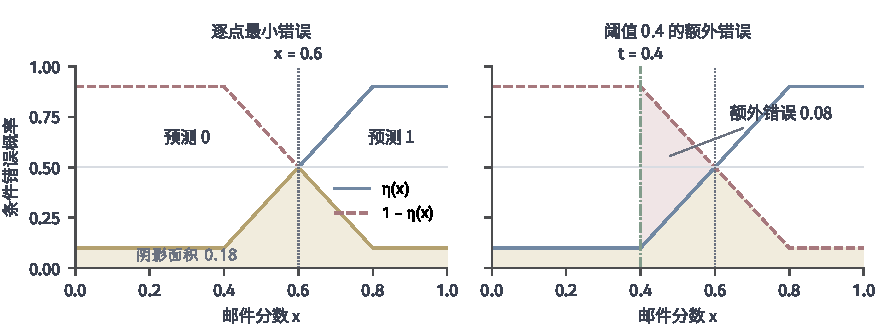
\includegraphics[width=150mm]{figures/06-foundations/02-learning-theory/matplotlib/lt4-bayes-eta/figure.pdf}
 \caption{贝叶斯风险的逐点计算。分数在$[0,1]$上均匀分布，实线为$\eta(x)=\mathbb P(y=1\mid x)$，虚线为$1-\eta(x)$。左图浅黄阴影为逐点最小错误$\min\{\eta,1-\eta\}$，面积即贝叶斯风险0.18；两条曲线在0.6处相交，贝叶斯分类器在其左侧预测0、右侧预测1。右图的阈值规则$h_{0.4}$在$[0.4,0.6)$上预测1，每个分数处多付出$(1-\eta)-\eta$，浅红区域面积为0.08。}
 \label{fig:lt4-bayes-eta}
\end{figure*}

右图比较一个非最优的阈值。$h_{0.4}$在$[0.4,0.6)$上预测1，错误概率是$1-\eta(x)$，而贝叶斯分类器在那里预测0，错误概率是$\eta(x)$；其余位置二者预测相同。多出的错误是两条曲线之间的面积
\[
 \int_{0.4}^{0.6}\bigl(1-2\eta(x)\bigr)\,\mathrm dx
 =\int_0^{0.2}(0.8-4u)\,\mathrm du=0.08,
\]
其中代入了$u=x-0.4$。于是$R_{\mathcal P}(h_{0.4})=0.18+0.08=0.26$。贝叶斯风险0.18任何分类器都去不掉，0.08则来自阈值放错了位置。

这个基准是当前输入信息允许的最佳水平，依赖输入表示和损失两者。换一种输入表示，例如在分数之外再读入发件人信息，同一封邮件的条件概率就变了，原来的0.18不能沿用。换一种损失也会改变基准。若把正常邮件误判为垃圾邮件的代价记为2、反方向的代价记为1，在$x$处预测1的条件期望损失是$2(1-\eta(x))$，预测0是$\eta(x)$，贝叶斯决策就改为在$\eta(x)\geq2/3$时才预测垃圾邮件；在上面的分布中，分界从0.6移到约0.683。

\subsection{近似误差与类内超额风险}
\label{sec:approximation-estimation}

再看假设空间的限制。设三个分数0.2、0.5、0.8各以概率$1/3$出现，标签分别确定为1、0、1。输入足以区分三者，贝叶斯风险为零；但单阈值产生不了“1、0、1”的变化：阈值不超过0.2时三封都判为垃圾，错在0.5；阈值在$(0.5,0.8]$中时错在0.2；其他位置错得更多。阈值空间的最低风险是$1/3$。这里缺的不是区分输入的信息，而是$\mathcal H$中能利用这些信息的规则。

有了贝叶斯风险这个最低基准，学习结果多出来的风险就可以在中间插入一层，拆成两段。第一段是因为把分类器限制在$\mathcal H$内而抬高的最低风险，称为\term{近似误差}（approximation error），等于类内最低期望风险减去贝叶斯风险；在输入表示和损失不变时，即使拥有无限数据、并能找到类内最优的规则，也消不掉它。第二段是算法在$\mathcal H$内的实际选择偏离类内最低风险的部分，也就是第~\ref{sec:pac-agnostic}节的超额期望风险；为与第一段对照，本书称它为类内超额风险，文献中也常称为\term{估计误差}（estimation error）。

对恰当输出$\hat h=A(S)\in\mathcal H$，在贝叶斯风险和输出风险之间插入类内下确界，就得到两段分解：
\begin{align}
 R_{\mathcal P}(\hat h)-R_{\mathcal P}^\star
 ={}&\left(\inf_{h\in\mathcal H}R_{\mathcal P}(h)-R_{\mathcal P}^\star\right)
 \label{eq:approximation-estimation-decomposition}\\
 &+\left(R_{\mathcal P}(\hat h)-\inf_{h\in\mathcal H}R_{\mathcal P}(h)\right).
 \notag
\end{align}
第一项是近似误差，第二项是类内超额风险。$\mathcal H$只含可测分类器，保证第一项非负；$\hat h\in\mathcal H$保证第二项非负。若允许非恰当输出，结果可能优于$\mathcal H$的下确界，第二项就可能为负；在上面的三点例子中，输出一条“0.2和0.8判垃圾、0.5判正常”的非阈值规则，风险为零，比阈值空间的下确界低$1/3$。

回到图~\ref{fig:lt4-bayes-eta}的分布：贝叶斯分类器本身就是阈值规则$h_{0.6}$，所以阈值空间的近似误差为零，$h_{0.4}$多出的0.08全部是类内超额风险。三点例子则相反，近似误差为$1/3$。一般情形两段都不为零。用一组教学数字串起三个水平：贝叶斯风险5\%，阈值空间的最低风险12\%，学到的阈值风险15\%。表达限制贡献7个百分点，类内选择贡献3个百分点，输出总共高于贝叶斯风险10个百分点，如图~\ref{fig:approximation-estimation-error}所示。若改变了输入表示，贝叶斯风险和候选空间都要重新确定，原来的5\%、12\%和7个百分点不能原样沿用。

\begin{figure}[htbp]
  \centering
  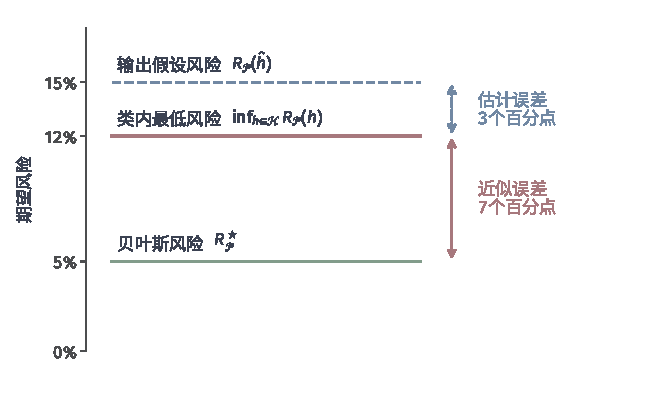
\includegraphics[width=112.000mm]{figures/06-foundations/02-learning-theory/matplotlib/learning-theory-error-decomposition/figure.pdf}
  \caption{风险的两段差距。教学设定中，贝叶斯风险为5\%，阈值空间最低风险为12\%，输出风险为15\%。前两者相差7个百分点，为实线表示的近似误差；后两者相差3个百分点，为虚线表示的类内超额风险（图中按文献常用名称标为估计误差）。}
  \label{fig:approximation-estimation-error}
\end{figure}

两段差距不应仅解释成“模型太简单”和“样本太少”。近似误差在空间固定时与样本量无关，但它也取决于输入表示和分布，不只取决于空间的大小。类内超额风险有可能随样本增多而缩小，但这取决于算法：始终返回同一个坏规则的算法，样本再多也不会改善；同样的样本量下，ERM和一个求解不充分的算法也可能相差很多。

扩大假设空间可以降低近似误差，却不自动降低实际算法的风险。正类由两个分离区间组成时，单阈值的近似误差不会因数据增加而消失；允许许多小区间的并以后，空间既能表达这种正类，也能把训练点一个个紧紧包住，未见的间隙反而可能被误判，类内超额风险更难控制。式~\eqref{eq:approximation-estimation-decomposition}的两段随空间一起变化，最终风险未必下降。这一取舍称为\term{偏差与复杂度的权衡}（bias--complexity trade-off）：“偏差”指空间的表达限制，“复杂度”指在有限样本中可靠选解的统计代价。

\subsection{经验求解误差怎样进入风险保证}
\label{sec:risk-comparison}

实际算法还未必能把训练错误降到最低。如果候选中训练错误最少的规则只错2封、算法返回的规则错5封，多出来的3次错误来自训练目标没有真正求解好。下面回到第~\ref{sec:pac-general-form}节的一般记号：比较决策空间为$\mathcal W$，损失$\ell(w,z)$，算法输出$\hat w=A(S)$，本小节始终设损失非负。\term{经验优化误差}（empirical optimization error）用两个经验风险之差计量：
\begin{equation}
  \Delta_{\mathrm{opt}}(S)
  =\hat R_S(\hat w)-\inf_{w\in\mathcal W}\hat R_S(w).
  \label{eq:empirical-optimization-error}
\end{equation}
恰当输出（$\hat w\in\mathcal W$）时它非负。它比较的是同一份样本上的两个量，而式~\eqref{eq:approximation-estimation-decomposition}的两项比较的是总体上的量；二者不在同一层次，不能把$\Delta_{\mathrm{opt}}$当作总体风险分解中的第三个等式项直接加进去。要把它计入输出风险，需要先把经验量和总体量连接起来。下面给出两种连接方式，后续各章反复使用。

\paragraph{高概率形式}
第一种方式要求一个事件：在这份样本上，比较空间中\emph{所有}决策的总体风险与经验风险都相差不多。所有决策同时满足，是因为输出$\hat w$由样本选出，事先不知道是哪一个。

\begin{theorem}[近似经验风险最小化的风险比较]
\label{thm:approximate-erm-risk}
设$\mathcal W$是非空比较决策空间，损失$\ell\geq0$，$\mathcal P$是$Z$上的分布，且每个
$w\in\mathcal W$的期望风险$R_{\mathcal P}(w)$有限。固定一份样本$S\in Z^n$及
$\alpha,\eta\geq0$。设学习算法在这份样本上的输出$\hat w=A(S)\in\mathcal W$满足
\begin{equation}
 \hat R_S(\hat w)\leq\inf_{w\in\mathcal W}\hat R_S(w)+\alpha,
 \label{eq:approximate-erm-condition}
\end{equation}
并且这份样本满足
\begin{equation}
 \sup_{w\in\mathcal W}\bigl|R_{\mathcal P}(w)-\hat R_S(w)\bigr|\leq\eta,
 \label{eq:uniform-deviation-event}
\end{equation}
则
\begin{equation}
 R_{\mathcal P}(\hat w)
 \leq\inf_{w\in\mathcal W}R_{\mathcal P}(w)+2\eta+\alpha.
 \label{eq:approximate-erm-risk}
\end{equation}
因此，若$S\sim\mathcal P^n$时式~\eqref{eq:uniform-deviation-event}以至少$1-\delta$的概率成立，而式~\eqref{eq:approximate-erm-condition}对每份样本都成立，则式~\eqref{eq:approximate-erm-risk}以至少$1-\delta$的概率成立。
\end{theorem}

\begin{proof}
固定任意参照$w\in\mathcal W$，依次用三次比较。输出$\hat w$属于$\mathcal W$，式~\eqref{eq:uniform-deviation-event}覆盖它，给出$R_{\mathcal P}(\hat w)\leq\hat R_S(\hat w)+\eta$；式~\eqref{eq:approximate-erm-condition}及$\inf_{v\in\mathcal W}\hat R_S(v)\leq\hat R_S(w)$给出$\hat R_S(\hat w)\leq\hat R_S(w)+\alpha$；式~\eqref{eq:uniform-deviation-event}用于参照$w$，给出$\hat R_S(w)\leq R_{\mathcal P}(w)+\eta$。连起来，
\[
 R_{\mathcal P}(\hat w)
 \leq\hat R_S(\hat w)+\eta
 \leq\hat R_S(w)+\alpha+\eta
 \leq R_{\mathcal P}(w)+\alpha+2\eta.
\]
左端不依赖$w$，对$w\in\mathcal W$取下确界即得式~\eqref{eq:approximate-erm-risk}。最后一句只是把这一确定性结论用于式~\eqref{eq:uniform-deviation-event}成立的事件。
\end{proof}

图~\ref{fig:lt4-risk-comparison-chain}用一组数字画出这三步：参照决策的总体风险为0.10，偏差至多$\eta=0.02$，求解容差$\alpha=0.01$。最坏情形下，参照的经验风险可以高到0.12，输出的经验风险再高出0.01，输出的总体风险又比它高0.02，合计0.15。两个$\eta$来自两次“总体—经验”之间的替换，一次用于参照、一次用于输出；$\alpha$来自近似求解。

\begin{figure}[htbp]
 \centering
 % 第4章：近似ERM的三步风险比较（高概率形式）。
% 教学数值：参照 w 的总体风险 R(w)=0.10；共同偏差事件内 eta = 0.02；求解容差 alpha = 0.01。
% 最坏情形链：R(h)=0.10 -> Rhat(h) <= 0.12 -> Rhat(hhat) <= 0.13 -> R(hhat) <= 0.15
% 纵坐标：风险 r 映射到 y = 4 + 800 (r - 0.095)（mm）。
\begingroup
\definecolor{FigureBlue}{HTML}{7188A3}\definecolor{FigureBlueFill}{HTML}{E5EAF0}
\definecolor{FigureGreen}{HTML}{829C8B}\definecolor{FigureGreenFill}{HTML}{E8EEE9}
\definecolor{FigureYellow}{HTML}{B4A16F}\definecolor{FigureYellowFill}{HTML}{F1ECDD}
\definecolor{FigureRed}{HTML}{A7787D}\definecolor{FigureRedFill}{HTML}{F0E5E6}
\definecolor{FigureInk}{HTML}{3B4252}\definecolor{FigureMuted}{HTML}{6B7280}
\begin{tikzpicture}[figure picture,x=1mm,y=1mm]
\def\r#1{\fpeval{4+800*(#1-0.095)}}
\node[figure heading] at (22,52) {总体风险};
\node[figure heading] at (62,52) {经验风险};
\draw[draw=FigureGrid,line width=.6pt] (22,2)--(22,49);
\draw[draw=FigureGrid,line width=.6pt] (62,2)--(62,49);
\foreach \v in {0.10,0.12,0.13,0.15}{\draw[draw=FigureGrid,line width=.4pt,dash pattern=on 1pt off 1pt] (6,\r{\v})--(78,\r{\v});
  \node[anchor=east,font=\figurefont\scriptsize,text=FigureMuted] at (6,\r{\v}) {$\v$};}
\node[circle,draw=FigureGreen,fill=FigureGreenFill,line width=.8pt,inner sep=1.3pt] (a) at (22,\r{0.10}) {};
\node[circle,draw=FigureGreen,fill=FigureGreenFill,line width=.8pt,inner sep=1.3pt] (b) at (62,\r{0.12}) {};
\node[circle,draw=FigureBlue,fill=FigureBlueFill,line width=.8pt,inner sep=1.3pt] (c) at (62,\r{0.13}) {};
\node[circle,draw=FigureBlue,fill=FigureBlue,line width=.8pt,inner sep=1.3pt] (d) at (22,\r{0.15}) {};
\node[anchor=east] at (20.5,\r{0.10}) {$R_{\mathcal P}(w)$};
\node[anchor=west] at (63.5,\r{0.12}) {$\hat R_S(w)$};
\node[anchor=west] at (63.5,\r{0.13}) {$\hat R_S(\hat w)$};
\node[anchor=east] at (20.5,\r{0.15}) {$R_{\mathcal P}(\hat w)$};
\draw[figure flow] (a)--node[figure edge label,pos=.5,below right=-.5mm] {$+\eta$} (b);
\draw[figure flow] (b)--node[figure edge label,left] {$+\alpha$} (c);
\draw[figure flow] (c)--node[figure edge label,pos=.5,above right=-.5mm] {$+\eta$} (d);
\node[figure note,anchor=west] at (82,\r{0.125}) {共同偏差事件\\内的最坏情形};
\end{tikzpicture}
\endgroup

 \caption{近似经验风险最小化的三步风险比较。左列为总体风险，右列为经验风险；箭头从参照决策$w$的总体风险出发，经它的经验风险、输出$\hat w$的经验风险，回到输出的总体风险。教学数值取$R_{\mathcal P}(w)=0.10$、$\eta=0.02$、$\alpha=0.01$，箭头旁标出每一步最多增加多少。}
 \label{fig:lt4-risk-comparison-chain}
\end{figure}

定理把学习保证分成两份互相独立的工作。统计分析负责提供覆盖数据依赖选择的偏差事件，即式~\eqref{eq:uniform-deviation-event}，并给出$\eta$、样本量和失败概率之间的关系：第~\ref{chap:binary-learnability}章用假设个数和VC维，第~\ref{chap:convex-learning-and-stability}章用Rademacher复杂度等工具。优化分析负责保证式~\eqref{eq:approximate-erm-condition}，并给出$\alpha$与计算量之间的关系。二分类中取$\eta=\varepsilon/4$、$\alpha=\varepsilon/2$，超额风险至多为$\varepsilon$；以后各章只说明怎样取得这两个条件，不再重复整段三步证明。

条件不足时不能直接代入。式~\eqref{eq:approximate-erm-condition}比较的是输出与\emph{全局}经验最优之间的差距。非凸目标上的梯度方法往往只能保证找到驻点，即梯度接近零的点；驻点的经验风险可能远高于下确界，这时$\alpha$没有被控制，定理也就给不出总体最优意义下的保证。反过来，偏差事件只覆盖$\mathcal W$；算法若输出$\mathcal W$之外的决策，第一步比较还需要把偏差控制推广到输出空间。

\paragraph{期望形式}
第二种方式不要求所有决策同时满足偏差界，而对重复抽取训练样本及算法随机性取期望。先引入两个平均量。对$S\sim\mathcal P^n$及独立的内部随机数$U$，记$\hat w=A(S,U)$，
\begin{align}
 G_n(\mathcal P)
 &=\mathbb E_{S,U}\bigl[R_{\mathcal P}(\hat w)-\hat R_S(\hat w)\bigr],
 \label{eq:expected-generalization-gap}\\
 O_n(\mathcal P)
 &=\mathbb E_{S,U}\Bigl[\hat R_S(\hat w)-\inf_{w\in\mathcal W}\hat R_S(w)\Bigr].
 \label{eq:expected-optimization-error}
\end{align}
$G_n$是期望泛化差，只涉及算法实际交出的输出；$O_n$是平均经验优化误差。

为什么不能直接把$\mathbb E_S\hat R_S(\hat w)$换成$\mathbb E_SR_{\mathcal P}(\hat w)$？对一个固定、与样本无关的决策$w$，$\mathbb E_S\hat R_S(w)=\frac1n\sum_i\mathbb E\,\ell(w,z_i)=R_{\mathcal P}(w)$，经验风险是无偏的。但$\hat w$由样本选出，这个等式一般不成立：第~\ref{sec:memorization-counterexample}小节的记忆规则每次的训练错误都是0，总体风险却都是0.4，期望泛化差为0.4。所以比较时只能把无偏性用在固定的参照决策上，再把输出与参照之间的差用加入并减去经验风险的办法连接起来。

\begin{theorem}[期望风险比较]
\label{thm:expected-risk-comparison}
设损失$\ell\geq0$，$\mathcal W$非空，每个$w\in\mathcal W$的期望风险有限；$S\sim\mathcal P^n$，
$U$独立于$S$，$\hat w=A(S,U)\in\mathcal W_{\mathrm{out}}$，$R_{\mathcal P}(\hat w)$与
$\hat R_S(\hat w)$可积，且$\inf_{w\in\mathcal W}\hat R_S(w)$作为$S$的函数可测（在第~\ref{sec:measurability-convention}段的约定下成立）。
\begin{enumerate}
 \item 平均输出风险满足
 \begin{equation}
  \mathbb E_{S,U}R_{\mathcal P}(\hat w)
  \leq\inf_{w\in\mathcal W}R_{\mathcal P}(w)+G_n(\mathcal P)+O_n(\mathcal P).
  \label{eq:expected-risk-comparison}
 \end{equation}
 \item 设对分布族$\mathfrak P$中每个$\mathcal P$，超额风险$R_{\mathcal P}(\hat w)-\inf_{w\in\mathcal W}R_{\mathcal P}(w)$几乎必然非负（恰当输出时自动成立），并且存在不依赖于$\mathcal P$的数列$b_n\to0$，使一切$\mathcal P\in\mathfrak P$都满足$G_n(\mathcal P)+O_n(\mathcal P)\leq b_n$。则对任意$\varepsilon,\delta\in(0,1)$，取$n_0$使$n\geq n_0$时$b_n\leq\varepsilon\delta$，便对一切$\mathcal P\in\mathfrak P$及$n\geq n_0$有
 \[
  \mathbb P_{S,U}\Bigl(R_{\mathcal P}(\hat w)\leq\inf_{w\in\mathcal W}R_{\mathcal P}(w)+\varepsilon\Bigr)\geq1-\delta,
 \]
 即该算法相对$\mathfrak P$满足定义~\ref{def:general-pac-learnability}的PAC保证。
\end{enumerate}
\end{theorem}

\begin{proof}
固定任意参照$w\in\mathcal W$。在输出与参照之间加入并减去三个经验量：
\[
 \begin{aligned}
 R_{\mathcal P}(\hat w)-R_{\mathcal P}(w)
 ={}&\bigl[R_{\mathcal P}(\hat w)-\hat R_S(\hat w)\bigr]
   +\Bigl[\hat R_S(\hat w)-\inf_{v\in\mathcal W}\hat R_S(v)\Bigr]\\
 &+\Bigl[\inf_{v\in\mathcal W}\hat R_S(v)-\hat R_S(w)\Bigr]
   +\bigl[\hat R_S(w)-R_{\mathcal P}(w)\bigr].
 \end{aligned}
\]
四项都可积：前两项由假设可积；$0\leq\inf_{v\in\mathcal W}\hat R_S(v)\leq\hat R_S(w)$，而$\mathbb E_S\hat R_S(w)=R_{\mathcal P}(w)<\infty$。第三项按下确界的定义不大于零。第四项中$w$固定、与样本无关，由经验风险的无偏性，其期望为零。对两边取期望，第一、二项的期望分别是$G_n(\mathcal P)$与$O_n(\mathcal P)$，于是
\[
 \mathbb E_{S,U}R_{\mathcal P}(\hat w)-R_{\mathcal P}(w)\leq G_n(\mathcal P)+O_n(\mathcal P).
\]
对$w\in\mathcal W$取下确界，得到式~\eqref{eq:expected-risk-comparison}。

对第二部分，令$Q=R_{\mathcal P}(\hat w)-\inf_{w\in\mathcal W}R_{\mathcal P}(w)$。按假设$Q\geq0$几乎必然成立，由第一部分$\mathbb EQ\leq G_n(\mathcal P)+O_n(\mathcal P)\leq b_n$。对非负随机变量用Markov不等式，
\[
 \mathbb P(Q>\varepsilon)\leq\mathbb P(Q\geq\varepsilon)\leq\frac{\mathbb EQ}{\varepsilon}\leq\frac{b_n}{\varepsilon}\leq\delta,
 \qquad n\geq n_0.
\]
$n_0$只由$b_n$、$\varepsilon$和$\delta$确定，不依赖$\mathcal P$，所以结论对$\mathfrak P$中的一切分布统一成立。
\end{proof}

两个定理依据的是不同的推理。高概率形式依赖一个共同偏差事件，所以要控制整个$\mathcal W$上的上确界，代价是两个$\eta$；期望形式依赖期望的线性和固定参照的无偏性，参照一侧不需要任何一致控制，剩下的$G_n$只关于算法实际交出的输出。第~\ref{chap:convex-learning-and-stability}章的稳定性和信息依赖方法正是直接控制$G_n$，不经过整个空间的上确界。

期望形式的代价在置信度上。Markov不等式要求平均超额风险低于$\varepsilon\delta$，样本量随$1/\delta$增长，而高概率形式通常只随$\log(1/\delta)$增长。用第~\ref{sec:pac-sample-complexity}小节的教学分布比较：零错误阈值的平均风险至多$2/n$，经Markov不等式要求$2/n\leq\varepsilon\delta$，取$\varepsilon=0.05$、$\delta=0.01$得$n\geq4000$；直接用尾概率界只需$n\geq104$。所以能用高概率界时，Markov只是一条备用路线。

第二部分的两个条件都不能省。若输出可以优于比较空间，$Q$可能取负值，Markov不等式不再适用。数列$b_n$必须对整个分布族统一：如果只知道对每个固定的$\mathcal P$都有$G_n(\mathcal P)+O_n(\mathcal P)\to0$，而收敛速度随$\mathcal P$变化，得到的$n_0$就依赖未知分布，只能推出第~\ref{sec:pac-sample-complexity}小节所说的一致性，不能推出分布无关的PAC保证。

\section{模型选择}
\label{sec:model-selection}

上一节说明，候选空间的选择同时影响近似误差和类内超额风险，二者此消彼长。实践中常有一列逐渐丰富的候选空间，例如让$\mathcal H_k$允许至多$k$个区间的并作为判为垃圾邮件的分数范围，$\mathcal H_1\subseteq\mathcal H_2\subseteq\cdots$。本节讨论怎样在它们之间选择，以及选择本身为什么也需要统计上的保护。两种基本思路使用不同的证据：验证选择另留一批数据直接比较，结构风险最小化则在同一批训练数据上加入复杂度代价。

\subsection{验证选择与独立测试}
\label{sec:validation-model-selection}

如果嵌套的假设空间逐渐扩大、每次又都精确最小化经验风险，训练误差只会持平或下降：更大的空间至少保留了前一个空间的全部候选，总能把训练样本拟合得一样好或更好，包括拟合其中的偶然性。所以训练误差的下降本身无法判断未来误差的走势。要比较不同复杂度或其他超参数，就需要一批不参与参数拟合的\term{验证样本}（验证样本为什么不能再当测试用，见第~\ref{sec:experience-data-boundary}节）。若验证样本独立于训练过程、且与未来数据同分布，那么对某个\emph{固定}的模型，验证误差是未来误差的无偏估计。

选择本身却会引入偏差。设有20个候选，它们的真实错误率都是10\%，每个候选在各自独立的200封验证邮件上评估，验证误差就是错误封数除以200，围绕10\%随机波动，标准差约为$\sqrt{0.1\times0.9/200}\approx0.021$。图~\ref{fig:lt4-validation-optimism}是重复20000次的模拟：任取其中一个候选，它的验证误差平均为0.100，确实无偏；但挑出20个中验证误差最小的那个，它的验证误差平均只有0.062，在约86\%的重复中不超过0.07。被选中的候选并不比其他候选更好，它们的真实错误率完全相同；偏低的只是“它被选中”这件事附带的随机波动。候选越多，偶然偏低的机会越大，最小值的乐观偏差也越大。

\begin{figure}[htbp]
 \centering
 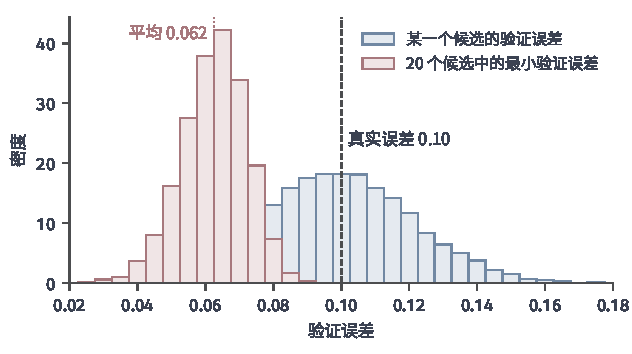
\includegraphics[width=107mm]{figures/06-foundations/02-learning-theory/matplotlib/lt4-validation-optimism/figure.pdf}
 \caption{从20个同样好的候选中取最小验证误差的乐观偏差。每个候选的真实错误率都是0.10，各在200个独立验证观测上评估；模拟重复20000次（随机种子20261030）。浅蓝直方图为任一固定候选的验证误差，以真实误差为中心；浅红直方图为20个验证误差中的最小值，平均约0.062。}
 \label{fig:lt4-validation-optimism}
\end{figure}

因此，最终评价必须覆盖“调参并选择模型”的整个流程，而不只是选中之后的那个模型（多次比较的统计含义可参考\BookVolumeRef{vol:mathematical-preliminaries-lower}{卷2《数学准备：概率、因果与决策》}）。实践中通常把数据分成三份，各承担一种作用：训练样本用来在每个候选空间内拟合参数；验证样本用来比较候选、确定$\hat k$与其他超参数；锁定整个流程以后，再用独立的\term{测试样本}评价最终结果。图~\ref{fig:learning-model-selection}用教学曲线展示这种分工：训练误差持续下降时，验证误差可能转而回升，合适的复杂度由验证误差的最低点确定，实际曲线也未必只有一个谷底。验证样本已经参与选择，它上面的最小误差同样带有上面所说的乐观偏差；如果继续看着测试误差改模型，测试样本也参与了选择，这次“独立评价”就失去了意义。

\begin{figure}[htbp]
  \centering
  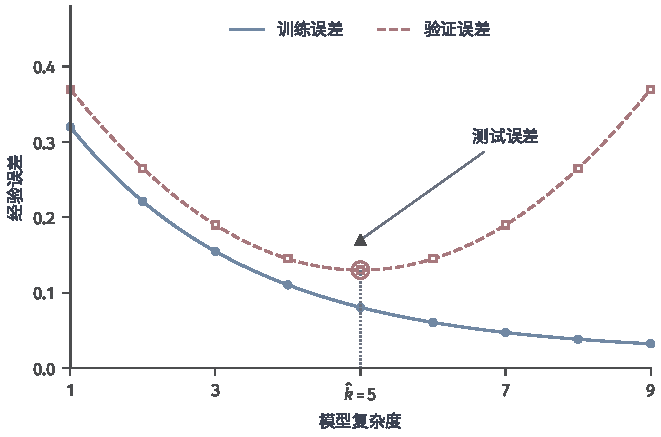
\includegraphics[width=112.000mm]{figures/06-foundations/02-learning-theory/matplotlib/learning-theory-model-selection/figure.pdf}
  \caption{教学示意中的验证选择与独立测试。实线圆点为训练误差，虚线方块为验证误差，圆环的最低验证误差确定$\hat k$。三角形仅为锁定模型后的一次测试评价，未参与选择，故不连成测试曲线。所有数值均为构造示意。}
 \label{fig:learning-model-selection}
\end{figure}

\subsection{结构风险最小化的目标}
\label{sec:srm-objective}

验证选择需要额外的数据。能否只用训练样本，在嵌套空间之间作出有依据的选择？先看两种极端做法各遗漏了什么。单纯选训练误差最低者，总会偏向更丰富的空间，忽视了类内超额风险随空间扩大而增加的统计代价；始终选最简单的空间，又忽视了它可能留下的较大近似误差。我们需要一条规则，同时顾及表达限制和有限样本下的选择代价。

两段误差都依赖未知分布，无法直接计算，能计算的只有经验风险。\term{结构风险最小化}（structural risk minimization, SRM）的思想是在经验风险之外加上一项随空间复杂度增长的惩罚，作为统计不确定性的抵扣，再在所有空间、所有候选中联合选择：
\[
 (\hat k,\hat h)\in\argmin_{k\geq1,\,h\in\mathcal H_k}\bigl\{\hat R_S(h)+\operatorname{pen}_k\bigr\}.
\]
经验项衡量训练拟合的好坏，惩罚$\operatorname{pen}_k$衡量在第$k$个空间中由样本推断总体时的不确定性。惩罚太小可能选中偶然拟合的复杂规则，太大又可能留下简单空间的表达偏差。

惩罚不能随意设定，它要来自一个对\emph{全部}候选空间同时成立的偏差保证。原因与上一小节的乐观偏差相同：每个空间单独的失败概率都不超过$\delta$，并不能保证看过数据、再从中选出一个空间之后，总失败概率仍不超过$\delta$。所以SRM要把总的失败概率预先分配给各个空间，使所有空间以足够高的概率同时满足各自的偏差界；惩罚正是由这些偏差界确定的。

SRM与验证选择依据的证据不同，二者不能互相等同。SRM不另留数据，但必须先有适用于每个候选空间的风险补偿，这类补偿要用后续章节的容量工具才能建立；验证选择不需要这些理论界，却要用额外的数据比较，并承受选择带来的乐观偏差。失败概率怎样分配、惩罚项怎样从容量界构造，以及SRM的输出与“知道各空间总体风险时的最佳选择”相比只多出多少，统一放到第~\ref{sec:srm}节，在第~\ref{chap:convex-learning-and-stability}章建立通用风险工具之后证明。

\section{可计算PAC学习}
\label{sec:computable-pac}
\label{sec:pac-computation-requirements}

前面的PAC定义只把算法看成一个从样本到分类器的数学映射，回答的是“有限的信息是否足以可靠预测”。但存在这样一个映射，并不等于知道计算机怎样实现它。一句“返回期望风险最小的假设”没有给出找到它的程序；即使改成“返回经验风险最小的假设”，候选无穷多时也未必能在有限时间内完成。本节在统计保证之上分两层加入计算要求：训练和预测都能停机，得到\term{可计算学习}（computable learning）；样本量、训练时间、预测时间和输出长度还都有关于约定参数的多项式上界，得到\term{高效学习}（efficient learning）。无论加哪一层，原来的统计保证都必须仍然成立。第~\ref{chap:binary-learnability}章与第~\ref{chap:multiclass-learnability}章沿用这里的定义，只补充各自标签空间的特殊条件。

\subsection{输入与预测规则的有效表示}
\label{sec:effective-representation}

程序处理的是有限的符号串，所以计算训练和预测之前，必须先约定输入、标签和输出规则怎样编码。几种常见对象的情况不同。自然数输入可以写成二进制串，数值$x$约占$\log_2(x+1)$位；有限标签集$\{1,\ldots,K\}$中的标签约占$\log_2K$位，二分类标签只占一位。实数则不同：任意实数未必有有限的精确编码，连续输入上的任意精度运算要先约定精度或计算模型，例如只处理有限位有理数，不能默认把它当作一次常数时间操作计费。编码长度会影响读写、比较和求值的成本，所以计算成本不能只按观测条数衡量：两份同样含100条观测的样本，若一份的数值是三位数、另一份是三百位数，按位比较一次大小的代价就相差约百倍。

输出也要有约定的表示。学习程序不能交出一个“数学函数”，只能交出一段有限描述，例如一个编号或一段代码，再由一个统一的求值程序根据这段描述和输入算出标签。为此，本部分对表示提出以下要求。第一，允许输出的规则组成一个表示族，每条规则对应一个有限描述，并存在一个统一的求值程序，对每个合法描述和每个允许输入都停机并返回一个标签。第二，学习程序在每份允许的有限样本上都停机，并返回一个合法描述。第三，描述是否合法、两个标签是否相等都可以判定；否则程序连“预测是否等于真实标签”、也就是零一损失都算不出来。第四，允许输出的范围事先规定：要求输出属于$\mathcal H$的表示，或允许输出其他可求值的规则。

停机要求同时覆盖训练和使用两个环节。输出一段可能永不返回的代码，等于没有提供可用的预测规则；训练程序在某些样本上永不停机，也就没有交出任何结果。允许算法很慢、但最终能完成，就已经满足可计算性；多项式时间是在此之上的另一项要求。

\subsection{可计算PAC及可计算样本上界}
\label{sec:computable-pac-definition}

把上一小节的表示要求加到PAC保证上，就得到可计算PAC学习。下面的定义同时适用于二分类和多分类，确定性算法即可说明全部区别。

\begin{definition}[可计算PAC学习]
\label{def:computable-pac-learning}
固定输入空间$X$与标签空间$Y$的有效编码，两个标签是否相等可判定；固定假设空间$\mathcal H\subseteq Y^X$，以及允许输出规则的表示族$\mathcal H_{\mathrm{out}}$，后者带有一个统一的求值程序，对每个合法描述和每个$x\in X$停机并返回$Y$中的标签。若存在程序$A$满足：
\begin{enumerate}
 \item $A$在每份有限带标签样本$S$上停机，返回$\mathcal H_{\mathrm{out}}$中的一个合法描述；
 \item 对任意$\varepsilon,\delta\in(0,1)$存在有限的$m(\varepsilon,\delta)$，使任意$n\geq m(\varepsilon,\delta)$及任意$X\times Y$上的分布$\mathcal P$都有
 \[
  \mathbb P_{S\sim\mathcal P^n}\Bigl\{
  R_{\mathcal P}(A(S))\leq\inf_{h\in\mathcal H}R_{\mathcal P}(h)+\varepsilon
  \Bigr\}\geq1-\delta,
 \]
\end{enumerate}
则称$\mathcal H$是不可知\term{可计算PAC可学习的}（computably PAC learnable），简称CPAC可学习。把分布限制为对$\mathcal H$可实现的分布、并把风险要求改为$R_{\mathcal P}(A(S))\leq\varepsilon$，得到可实现版本。$\mathcal H_{\mathrm{out}}$就是$\mathcal H$的表示时称为恰当CPAC，允许输出其他可求值规则时称为非恰当CPAC。
\end{definition}

这些约束改变的是程序与输出，不取代原有的统计成功标准：第二条与定义~\ref{def:realizable-pac}、定义~\ref{def:agnostic-pac}完全相同，第一条才是新增要求。所以每个CPAC可学习的假设空间都是PAC可学习的。使用时必须说明采用可实现还是不可知版本、恰当还是非恰当输出；引用文献结论时也要先确认对方使用的约定，不能混用。

能逐个枚举假设，并不等于能在有限时间内完成ERM。若假设空间是有限个可执行程序组成的列表，可以逐个计算经验风险，再选出最小者。若假设空间无限但可以逐个枚举，这种做法就无法结束：在有噪声的样本上，当前最好的假设经验风险可能仍大于零，尚未检查的假设中可能有更小的，程序无法确认已经找到最小值。

训练可执行也不代表能算出充分样本量。定义只要求$m(\varepsilon,\delta)$\emph{存在}：给定一份有限样本，程序能完成训练；但使用者事先要准备多少样本，定义并没有要求程序能告诉他。若进一步要求存在一个程序，能根据有理数$\varepsilon,\delta$算出一个充分的样本量，就得到文献中的strong CPAC。这里的strong只指样本量上界可以算出，与精度高低无关，也与第~\ref{sec:boosting}节提升方法中把弱学习器加工成任意精度学习器的“强学习”不是一回事。基本CPAC不自动满足这一项额外要求，相关的刻画与分离结果见Delle Rose等人的工作\scite{dellerose2023}。本章只建立这些区别：二分类中的有效VC维、多分类中的可计算Natarajan维，以及它们与CPAC的关系，分别留给第~\ref{sec:computable-binary-learning}节和第~\ref{sec:computable-multiclass-learning}节，这里不预设它们之间的等价。

\subsection{高效学习与资源核算}
\label{sec:efficient-pac-resources}

程序能停机，仍可能慢到无法使用。有限个假设总可以穷举，但穷举可能需要指数时间。设假设由$d$个比特索引，共有$2^d$个成员、每个都能在多项式时间内求值，那么逐一计算经验风险要检查指数多个候选。而定理~\ref{thm:finite-realizable-pac}给出的可实现充分样本量只按
\[
 \frac{d\log2+\log(1/\delta)}{\varepsilon}
\]
增长。样本量上的线性和穷举规模上的指数并不矛盾，它们衡量的是两种不同成本：前者是信息成本（需要多少数据），后者是搜索成本（找到好假设要多少计算）。这个比较只说明穷举不够高效，并没有排除利用结构设计更快算法的可能。

\begin{definition}[高效PAC学习]
\label{def:efficient-pac-learning}
高效PAC学习（efficient PAC learning）要求在满足PAC期望风险保证的同时，样本量、训练计算量、输出表示长度及输出分类器的预测计算量都有多项式上界。为明确规模依赖，考虑由参数$d$描述的一族假设空间$\mathcal H_d$，并约定观测编码长度上界为$b$。本书采用的高效性约定要求存在统一程序和固定多项式$p,q$，使所需样本量及训练时间分别满足
\begin{equation}
 \begin{aligned}
 m_{\mathcal H_d}(\varepsilon,\delta)
 &\leq p\bigl(d,b,1/\varepsilon,\log(1/\delta)\bigr),\\
 T_{\mathrm{train}}
 &\leq q\bigl(n,d,b,1/\varepsilon,\log(1/\delta)\bigr).
 \end{aligned}
 \label{eq:efficient-pac-resources}
\end{equation}
学习程序把$d,\varepsilon,\delta$及样本编码作为输入；若$\varepsilon,\delta$只通过预先给定的
样本量体现，也必须明确这一接口。输出分类器属于预先规定、可统一求值的表示族，其描述长度
及在新的预测输入上的求值时间应被$d$、$b$和输入编码长度的某个固定多项式所控制，不能仅把任意
程序的短代码长度当作预测高效的依据。若这族假设空间还由目标描述长度等量参数化，也须将
它们明确列入规模变量。
\end{definition}

以多项式作为“高效”的界线，是计算复杂性理论的通行约定：多项式增长在规模加倍时只让成本乘上一个固定倍数，指数增长则让成本随规模每增加一点就成倍膨胀；这条界线还不随编码细节的合理变化而改变。规模参数$d$由具体问题约定，不一定是特征维数；编码长度$b$则保证长数值的读写和比较都计入成本；精度$1/\varepsilon$与置信度$\log(1/\delta)$按定义中的形式计入。统一多项式还要求次数不随$d$增长。不同文献有时用$1/\delta$、有时用$\log(1/\delta)$描述资源，引用时必须核对。即使满足多项式上界，很大的常数或很高的次数也可能让实际计算难以承受；多项式界不等于在任意规模上都有可接受的耗时。

高效算法不一定要精确求解ERM。由定理~\ref{thm:approximate-erm-risk}，若用多项式个样本能使式~\eqref{eq:uniform-deviation-event}以$\eta\leq\varepsilon/4$成立，用多项式训练时间能达到$\alpha\leq\varepsilon/2$，并且输出长度和预测时间也是多项式，就得到一条通向高效不可知PAC学习的充分路线。某个精确ERM难以计算，也不排除其他近似算法或非恰当算法可行。

穷举是最坏的做法，问题若有结构，搜索可以快得多。整数阈值就是一例。设输入是$1,\ldots,M$中的整数，假设为$h_t(x)=\mathbb I\{x\geq t\}$，$t\in\{1,\ldots,M+1\}$。候选有$M+1$个，而$M$的编码只占约$\log_2M$位，逐个检查对编码长度而言是指数代价。关键观察是：阈值在两个相邻的已见输入之间移动时，样本上的预测不变，只有越过某个已见输入时才会改变，所以只需检查至多$n+1$个切分位置。

图~\ref{fig:lt4-integer-threshold-scan}用一份7条观测的样本演示。按输入排序并合并重复后，不同的输入是2、5、6、9、11，其中5处有一正一负两条观测。切分$c_0$位于所有输入左侧，全部判为正，错在3个负例上；每向右越过一个输入，越过的负例改判为负、错误数减一，越过的正例改判为负、错误数加一。依次得到错误数3、2、2、3、4、3。越过5时一正一负相抵，错误数不变。最少错误为2，在$c_1$、$c_2$并列，按“选较小阈值”的约定取$c_1$，例如$t=3$。

\begin{figure*}[htbp]
 \centering
 % 第4章：整数阈值的排序扫描。
% 样本（已按输入排序并合并重复）：x=2:负1；x=5:正1、负1；x=6:正1；x=9:正1；x=11:负1。
% 切分 c_k 位于第 k 个与第 k+1 个不同输入之间，左侧判 0、右侧判 1。
% 错误数 = 左侧正例数 + 右侧负例数：c_0..c_5 依次为 3, 2, 2, 1, 0+... 见下表：
%   c0 (t<=2): 左正0 + 右负3 = 3
%   c1 (2<t<=5): 0 + 2 = 2
%   c2 (5<t<=6): 1 + 1 = 2
%   c3 (6<t<=9): 2 + 1 = 3
%   c4 (9<t<=11): 3 + 1 = 4
%   c5 (t>11): 3 + 0 = 3
% 最少错误 2，在 c1 与 c2 并列；选较小阈值得到 t = 3（与 t=3,4,5 等价）。
% 越过负例错误数减1，越过正例加1；x=5 同时含正、负，越过它净变化为 0。
\begingroup
\definecolor{FigureBlue}{HTML}{7188A3}\definecolor{FigureBlueFill}{HTML}{E5EAF0}
\definecolor{FigureGreen}{HTML}{829C8B}\definecolor{FigureGreenFill}{HTML}{E8EEE9}
\definecolor{FigureYellow}{HTML}{B4A16F}\definecolor{FigureYellowFill}{HTML}{F1ECDD}
\definecolor{FigureRed}{HTML}{A7787D}\definecolor{FigureRedFill}{HTML}{F0E5E6}
\definecolor{FigureInk}{HTML}{3B4252}\definecolor{FigureMuted}{HTML}{6B7280}
\begin{tikzpicture}[figure picture,x=1mm,y=1mm]
\def\u{7.5}
\draw[draw=FigureStroke,line width=.75pt,-{Stealth[length=1.6mm]}] (\u*0.5,10)--(\u*12.6,10);
\foreach \v in {1,...,12}{\draw[draw=FigureStroke] (\u*\v,9.3)--(\u*\v,10.7);\node[anchor=north,font=\figurefont\scriptsize,text=FigureMuted] at (\u*\v,9) {$\v$};}
\node[anchor=west] at (\u*12.6,10) {$x$};
% observations: negatives hollow blue, positives filled red, stacked
\foreach \x/\yy in {2/14,5/14,11/14}{\draw[draw=FigureBlue,fill=FigureBlueFill,line width=.7pt] (\u*\x,\yy) circle(1.3);}
\foreach \x/\yy in {5/17.4,6/14,9/14}{\draw[draw=FigureRed,fill=FigureRed,line width=.7pt] (\u*\x,\yy) circle(1.3);}
% cut positions and error counts
\foreach \c/\xc/\e in {0/1.2/3,1/3.5/2,2/5.5/2,3/7.5/3,4/10/4,5/11.6/3}{
  \draw[draw=FigureMuted,line width=.5pt,dash pattern=on 1pt off 1pt] (\u*\xc,11.4)--(\u*\xc,21);
  \node[font=\figurefont\scriptsize] at (\u*\xc,24) {$c_{\c}$};
  \node at (\u*\xc,1.8) {$\e$};}
\fill[FigureYellowFill] (\u*3.5-3,-0.6) rectangle (\u*5.5+3,4.2);
\node at (\u*3.5,1.8) {$2$};\node at (\u*5.5,1.8) {$2$};
\node[anchor=east] at (\u*0.9,1.8) {错误数};
\node[figure note,anchor=west] at (\u*12.6,19) {空心：负例\\实心：正例};
\end{tikzpicture}
\endgroup

 \caption{整数阈值的排序扫描。7条构造的观测画在数轴上，空心点为负例，实心点为正例，输入5处有一正一负。虚线$c_0,\ldots,c_5$是全部需要检查的切分位置，切分左侧判0、右侧判1；下方为各切分的训练错误数。每越过一个输入只需按其正负例个数增减一次计数，浅黄底标出最少错误的两个并列切分。}
 \label{fig:lt4-integer-threshold-scan}
\end{figure*}

一般做法分三步。先把样本按输入排序、合并重复输入，记下每个输入处正、负标签各有多少。再从左到右扫描每个切分位置：切分左侧的正标签被判为负，右侧的负标签被判为正，二者之和就是该切分的训练错误数，每移动一个位置只需按越过输入处的计数增减一次。最后选错误最少的切分。排序需要$O(n\log n)$次比较，扫描需要$O(n)$次累计；比较一次输入约需$\log_2(M+1)$位操作，计数约需$\log_2(n+1)$位；输出是一个阈值，长度约$\log_2(M+2)$位，预测只需一次比较。总代价是$n$与$\log M$的多项式，而不是$M$的多项式。这里只借此说明结构怎样把对全部阈值的搜索变成对样本切分位置的比较，以及成本怎样核算；结合有限假设空间的样本界说明它满足高效PAC要求，放到第~\ref{chap:binary-learnability}章相应样本界之后。

固定风险目标、表示方式和输出范围后，三层要求之间有包含关系：满足高效PAC一定满足可计算PAC，满足可计算PAC一定满足定义~\ref{def:general-pac-learnability}的统计意义上的PAC；反方向都需要补充条件。本章出现的几组概念限制的是学习的不同侧面：可实现与不可知限制数据分布，恰当与非恰当限制输出范围，可计算与高效限制执行方式。它们可以组合使用，但不能用其中一项代替另一项。

\FloatBarrier

\section{研究内容}
\label{sec:learning-theory-research-content}

前面几节已经说明，训练误差较小还不能保证未来风险较小。候选模型可能遗漏所需的关系，训练可能没有充分求解经验目标，依据有限样本选出的结果也可能只适合这批样本。这三种情况分别对应近似误差、经验优化误差和类内超额风险。理论研究据此分别考察表达能力、优化过程和泛化性，再说明这些结论怎样共同支持一个学习保证。三者回答的问题不同，却作用于同一个输出，不是先后进行、互不相干的三个学习阶段。

\subsection{表达能力}
\label{sec:research-expressivity}

首先要问：在当前输入表示和候选范围内，是否存在风险足够低的规则？这包括两个层次。当前输入是否保留了预测所需的信息，由贝叶斯风险刻画：邮件若只保留词数和链接数，模型就不能利用发件人或语境中的差异，再大的模型也恢复不了输入中已经丢失的信息。即使输入信息充分，受限的候选空间也可能无法表达所需关系，这部分由近似误差刻画。表达能力研究据此说明给定函数类能够表示或逼近哪些目标，以及达到指定精度需要怎样的表示规模。

在输入、损失和分布固定时，扩大候选范围不会提高类内最低风险，却改变了有限样本下辨别和选择的难度。理论因此还要交代输出允许落在哪个空间、标签有怎样的结构，以及这些条件怎样影响学习。二分类和多分类章节考察候选空间在有限个输入上能实现多少种标签组合，并说明同一种容量判断为何不能直接用于不同的标签空间；深度学习章节考察网络架构及训练中形成的特征；迁移学习章节还要判断已有表示是否保留了目标任务所需的信息。

\subsection{优化过程}
\label{sec:research-optimization}

存在合适的候选以后，还要问算法能否找到它。经验风险最小化规定了选择目标，却没有直接给出求解程序。优化研究考察实际训练算法能否找到经验目标足够小的输出，以及步长、初始化、曲率和随机更新怎样影响训练过程。这里要区分几种不同的结论：目标值下降、到达驻点、接近全局最优，以及在多个最优解之间选择了哪一个。它们回答不同的问题，不能用梯度变小直接推出学习成功；第~\ref{sec:risk-comparison}节的风险比较要求的是相对全局经验最优的容差。

迭代步数也不等于全部计算代价：每步运算、数值精度、存储和预测都要计入，这正是第~\ref{sec:computable-pac}节的资源核算。二分类与多分类章节在有效表示下讨论可计算与高效学习；一般学习章用正则化与梯度训练连接经验求解误差和风险，并分析梯度方法对解的选择；深度学习章节进一步检查网络参数化与特征变化的条件。它们共同区分“好解存在”“程序能够返回结果”和“资源预算足以求出结果”。

\subsection{泛化分析}
\label{sec:research-generalization}

算法充分拟合训练样本之后，还要问所得规则在新观测上的风险有多大。泛化分析可以控制训练评价与总体评价的偏离，也可以直接控制相对比较空间的超额风险，并给出误差、失败概率与样本量之间的关系。保证必须覆盖由数据选择模型的过程，不能只证明一条预先固定的规则可靠。三类依据各有侧重：函数类的容量考察全部候选给数据依赖选择留下的余地，稳定性考察替换一条样本引起的输出变化，信息方法考察训练数据与输出之间的依赖。它们给出的保证在概率形式（高概率或期望）和适用条件上各不相同，需要分别说明。

泛化结论还要与前两方面联系起来。较小的泛化差可以伴随很高的风险：在只含正常邮件的分布上，总把邮件判为垃圾的规则，经验风险和总体风险都为1，泛化差却为0。低经验风险也可能只是拟合了当前样本。完整的保证还需要合适的表达基准和实际的求解条件。数据来源改变后，训练风险与目标风险之间又需要额外的联系；第~\ref{chap:transfer-learning-theory}章据此讨论迁移、历史表现的保持和有限记忆，而不直接沿用同分布下的结论。

表~\ref{tab:learning-theory-chapter-questions}列出后续各章如何落实这三类问题。每章固定一组学习对象和信息条件，再分析能够得到什么保证；同一章可以同时涉及多个问题。

\begin{table*}[htbp]
  \centering
  \small
  \begin{tabularx}{\linewidth}{@{}lX@{}}
    \toprule
    \textbf{后续章节} & \textbf{主要研究问题} \\
    \midrule
    第~\ref{chap:binary-learnability}章：二分类 & 候选分类规则的组合结构怎样控制样本量并刻画可学习性；统计保证何时能由停机、高效的程序实现。 \\
    第~\ref{chap:multiclass-learnability}章：多分类 & 标签空间扩大后，哪些组合维度分别控制一致收敛与可学习性；有限与一般标签空间的结论有何不同。 \\
    第~\ref{chap:convex-learning-and-stability}章：一般学习 & 一般损失下怎样用复杂度、压缩、稳定性和信息依赖控制泛化；模型选择、集成学习、正则化和梯度下降能得到什么风险保证。 \\
    第~\ref{chap:deep-learning-theory}章：深度学习 & 网络怎样训练、怎样选解、怎样形成特征；训练所得网络的风险怎样评价；双重下降等现象怎样解释。 \\
    第~\ref{chap:transfer-learning-theory}章：迁移与持续学习 & 分布或任务变化后信息是否足够；旧数据不可重访时，目标与历史风险需要多少样本和记忆才能控制。 \\
    \bottomrule
  \end{tabularx}
  \caption{理论研究问题与后续章节的对应关系。各章改变的对象和条件不同，不以同一种保证替代全部学习要求。}
  \label{tab:learning-theory-chapter-questions}
\end{table*}

\FloatBarrier

\section{研究历史}
\label{sec:learning-theory-research-history}

学习理论的发展，可以沿着“需要解释什么、现有条件还缺什么”来理解。下面按主要研究问题的扩展划分四个阶段，说明每一阶段增加了哪些分析对象，以及已有结论留下了什么边界。年份表示相应方向集中发展的时期，彼此有重叠；新方向通常补充已有工具，并不意味着较早的路线被取代。最后一个阶段介绍截至2026年10月与本部分直接相关的研究课题，所举代表工作只覆盖各自设定，不构成适用于全部学习系统的统一理论。

\subsection{1970年代至1980年代：一致收敛与可学习性的形式化}
\label{sec:history-uniform-convergence}

早期统计推断已经研究估计误差和重复抽样，学习算法还带来一个选择问题：规则由样本选出，因而不能只分析一条事先固定的规则的频率估计，而要同时控制整个候选集合。Vapnik与Chervonenkis在1971年研究了一族事件的相对频率何时一致地收敛到各自的概率，并把这种一致收敛与这族事件在有限个点上能划分出多少种子集联系起来\scite{vapnik1971}。用后来称为VC维的量衡量分类规则能实现的二元划分，便可把候选类的丰富程度转成整个类的评价偏差保证，这正是第~\ref{sec:risk-comparison}节高概率比较所需的那类偏差事件。

Valiant在1984年从计算角度提出了可学习性的形式框架：学习器按规定的协议取得样本，须在多项式时间内输出一个以高概率近似正确的描述\scite{valiant1984}。精度、成功概率、数据取得方式和计算要求由此都进入了可学习性的正式问题。这一阶段形成了后续分析的基本语言：学习器先于未知分布确定，再用受控的样本量实现风险要求。它也把两类问题分开了：统计信息是否足够，与程序能否高效完成。统计上可学并不意味着存在高效算法，候选表示、信息取得方式和运行时间仍须分别分析。

\subsection{1990年代至2000年代：学习器构造与泛化分析的扩展}
\label{sec:history-constructions}

研究从判断一个假设空间能否学习，进一步转向怎样由已有学习器构造更强的学习器。Schapire在1990年证明，在分布无关的PAC模型中，一个概念类弱可学习当且仅当它强可学习：只要存在对每个分布都比随机猜测略好的学习算法，就能构造出达到任意精度的学习算法，证明本身给出了这种转换\scite{schapire1990strength}。这为提升算法提供了构造依据。它要求的是对每个分布都保持统一的优势，不能理解成任意单个分类器在一份数据上略优于猜测就足够。

研究对象扩展到实值得分、回归和一般损失之后，仅计二元划分就保留不了数值大小与分辨精度；阈值、尺度及样本上的函数值成为新的分析对象。Bartlett与Mendelson在2002年用Rademacher复杂度和高斯复杂度给出风险界，并研究了这些复杂度在函数类的组合下怎样变化\scite{bartlettmendelson2002}。这类依赖实际样本的容量估计，补充了按最坏输入位置计数的方法。

另一条线索直接分析随机预测器和具体算法。McAllester在1999年给出的PAC--Bayes定理，把预先选定的先验分布与依据数据选出的预测分布之间的差异纳入风险控制\scite{mcallester1999pacbayes}；Bousquet与Elisseeff在2002年以替换或删除一条观测时输出的变化定义算法稳定性，并据此建立了基于经验误差和留一误差的泛化界\scite{bousquetelisseeff2002}。两条路线分别控制分布相对参照的代价与算法对样本的敏感性，不是同一种算法性质的两种说法；它们都还须结合拟合程度和比较基准，才能完成学习保证。

\subsection{2010年代：训练轨迹、隐式偏置与宽网络近似}
\label{sec:history-training-dynamics}

分析逐步深入到实际的迭代过程：停止时刻、步长和更新规则会改变样本扰动的传播，也会改变多个低经验风险解之间的选择。Hardt、Recht与Singer在2016年对随机梯度方法给出稳定性界，界的大小由迭代步数和步长控制，凸情形与部分非凸情形分别有不同条件\scite{hardt2016sgd}。Soudry等人在2018年证明，在线性可分数据上用梯度下降训练无正则化的逻辑回归等模型，参数的方向收敛到最大间隔分类器的方向，且这种收敛很慢\scite{soudry2018implicit}。前者说明轨迹对样本的敏感性怎样进入泛化分析，后者说明没有显式正则项时优化过程仍偏向某类解；两者都只在各自的算法与数据条件下成立。

Jacot、Gabriel与Hongler在2018年引入神经切线核，证明在指定的无限宽极限下，网络函数在梯度下降中的演化由一个训练期间保持不变的核描述，训练可以在函数空间而不是参数空间中研究\scite{jacot2018ntk}。这把部分训练问题接到了较易分析的核方法上。这一近似的适用条件与有限宽、特征显著变化的情形不同；训练过程可解释、优化收敛与测试风险受控，仍是需要分别连接的三个结论。

\subsection{2020年代至当前：可执行刻画、特征形成与变化环境}
\label{sec:history-current}

当前课题之一是把统计刻画继续连接到样本效率和可执行的算法，而不只判断某种学习器存在。Brukhim等人在2022年证明，多分类的PAC可学习性由DS维刻画，而Natarajan维不能刻画一般标签空间上的可学习性，他们构造了Natarajan维为1却不可学习的类；其正面结果用到列表学习等多种算法构造，不再像二分类那样归结为ERM\scite{brukhim2022multiclass}。Gourdeau、Lechner与Urner在2025年研究有限标签空间上的可计算PAC学习，提出可计算的Natarajan维并证明它刻画了这一设定下的可计算可学习性\scite{gourdeau2025multiclass}。这些结果说明标签空间、输出约定和有效表示都会改变问题。另一个方向考察怎样利用实际算法的稳定性或信息依赖得到有用的风险控制。已有刻画与仍需针对具体设定分析的效率问题要分开看，DS维、样本压缩和信息量也不能当作可以无条件互换的标准。

另一组课题研究特征何时形成、训练误差已经很低之后为何还会出现泛化的变化，以及这种表示变化怎样影响新任务的学习与旧任务的保持。训练早已拟合、测试表现却在更晚才改善的现象称为\term{顿悟}（grokking）。Kumar等人在2024年用两层网络上的多项式回归给出了一条机制：网络先在初始特征下以近似核回归的方式拟合训练数据，之后才发生特征学习并找到泛化的解；延迟的程度取决于特征学习的速度，以及初始特征与目标函数的对齐程度\scite{kumar2024grokking}。Lyle等人在2025年把这种特征学习动力学与非平稳学习联系起来，提出促进特征学习的方法也可能有助于克服早期数据妨碍后续泛化的问题，并在顿悟、热启动训练和强化学习等设定中检验了提高有效学习率的做法\scite{lyle2025plasticity}。前者是受控模型中的机制分析，后者是由此出发的研究假说与跨任务实验；延迟泛化与持续学习都还没有统一的解释。第~\ref{chap:deep-learning-theory}章与第~\ref{chap:transfer-learning-theory}章分别从训练现象和变化环境两侧展开这些问题。

\section{本章小结}
\label{sec:statistical-framework-summary}

本章从“有限观测什么时候支持可靠预测”出发。要回答这个问题，先要写清楚一个学习保证在说什么。一个完整的保证必须固定允许的数据来源、比较空间与输出空间、损失、精度与置信度。数据独立同分布地取自一个未知来源；算法依据训练样本从候选中交出一条规则；规则用期望风险评价，而算法能计算的只是经验风险。PAC学习把这些要素放进一个量词顺序：先固定算法，再给定$\varepsilon$与$\delta$，样本门槛不能依赖未知分布，最后对允许分布族中的每个来源提出要求。可实现情形以零风险为基准，不可知情形以类内最低风险为基准。训练表现只是其中一项证据，平均风险趋于零或对每个分布分别收敛，都比分布无关的高概率保证弱。

归纳偏置是正面保证的前提。记忆反例说明，经验风险最小化本身不约束未见输入上的预测；没有免费的午餐定理进一步说明，若候选空间允许未见标签自由变化，任何算法都会在某个固定来源上以固定概率失败，原因是样本缺少标签信息，增加计算也补不回来。阈值规则之所以学得会，是因为一个已见标签就约束了许多未见位置。

归纳偏置也留下代价，风险因此分层。贝叶斯风险是当前输入与损失允许的最低水平，近似误差是候选空间的表达限制，类内超额风险是算法在空间内选得不够好的部分。经验优化误差位于样本层面，只能通过风险比较进入保证：高概率形式要求一个覆盖整个比较空间的偏差事件，给出“两次偏差加一次求解容差”；期望形式只用固定参照的无偏性，留下输出的期望泛化差，再在统一的平均界之下借Markov不等式转为PAC保证。验证选择与结构风险最小化分别用额外数据和同时成立的复杂度代价处理“看过数据再选模型”的偏差。可计算与高效学习则要求数学上的选解能由停机且资源受控的程序实际取得。

下一章固定二元标签和零一损失，先用有限候选的计数为风险比较提供偏差事件，证明有限假设空间可学习；再寻找适用于无限候选的结构尺度，并在有效表示下考察相应的程序能否停机、是否高效。

\paragraph{扩展阅读}
Shalev-Shwartz与Ben-David的\textit{Understanding Machine Learning}第2--5章展开了PAC、ERM和没有免费的午餐。读这些结果时可以核对各自的比较基准和“算法先于分布确定”的量词顺序，从而判断结论适用于哪一类学习问题\scite{shalevshwartz2014}。

Delle Rose等人的可计算PAC研究区分了“统计上存在”和“能有效找到见证”\scite{dellerose2023}：在有限输入集上，假设空间可能无法实现某种标签组合，但知道这种缺失组合存在，并不等于有一个有限时间程序能把它找出来作为见证返回。第~\ref{sec:computable-binary-learning}节会用定义和例子落实这一区别，阅读时可与原文的表示和输出约定对照。结构风险最小化的深入阅读随第~\ref{sec:srm}节的正式论证给出。
